% \documentclass[runningheads]{llncs}
% \pdfoutput=1
% \usepackage[utf8]{inputenc}
% \usepackage{graphicx}
% \usepackage{comment}
% \usepackage{biblatex}
% \usepackage{placeins}
% \usepackage{amsmath,amssymb,amsfonts,bm} % define this before the line numbering.
% \usepackage{color}
% \usepackage{booktabs}

% \usepackage{import}
% \usepackage{appendix}
% \usepackage[caption=false]{subfig}
% \usepackage{mathtools}
% \usepackage{wrapfig}
% \usepackage{hyperref}

% \def\ci{\perp\!\!\!\perp}
% \newcommand{\myles}[1]{\textcolor{blue}{\textbf{Myles:} #1}}
% \newcommand{\thomas}[1]{\textcolor{red}{\textbf{Thomas:} #1}}
% \newcommand{\oliver}[1]{\textcolor{magenta}{\textbf{Oliver:} #1}}
% \newcommand*\diff{\mathop{}\!\mathrm{d}}
% \def\httilde{\mbox{\tt\raisebox{-.5ex}{\symbol{126}}}}

% \addbibresource{references.bib}

% \begin{document}

% \pagestyle{headings}
% \mainmatter
% \def\ECCVSubNumber{5488}  % Insert your submission number here

% \title{Null-sampling for Interpretable \\and Fair Representations} % Replace with your title

% \titlerunning{Null-sampling for Interpretable and Fair Representations}
% \author{Thomas Kehrenberg \and
% Myles Bartlett \and
% Oliver Thomas \and \\
% Novi Quadrianto}
% \authorrunning{T. Kehrenberg et al.}
% \institute{Predictive Analytics Lab (PAL), University of Sussex, Brighton, UK
% \email{\{t.kehrenberg,m.bartlett,ot44,n.quadrianto\}@sussex.ac.uk}}
% \maketitle

% 70-150 words
\section{Abstract}
\noindent
% Training data often contains spurious correlations not reflected in the real world where a trained model will be deployed.
% Consequently, computer vision and machine learning systems can become over-reliant on these correlations for classifications.
% Instead of basing their output on those features which are semantically meaningful, the output can be based on these unintended relationships.
% This is undesirable for many reasons, among them limited generalisation and uncontrolled bias.
We propose to learn invariant representations, in the data domain, to achieve interpretability in algorithmic fairness. 
Invariance implies a selectivity for high level, relevant correlations w.r.t. class label annotations, and a robustness to irrelevant correlations with protected characteristics such as race or gender. 
We introduce a non-trivial setup in which the training set exhibits a strong bias such that class label annotations are irrelevant and spurious correlations cannot be distinguished.
To address this problem, we introduce an adversarially trained model with a \emph{null-sampling} procedure to produce invariant representations in the data domain.
To enable disentanglement, a partially-labelled \emph{representative} set is used.
By placing the representations into the data domain, the changes made by the model are easily examinable by human auditors.
We show the effectiveness of our method on both image and tabular datasets: Coloured MNIST, the CelebA and the Adult dataset.%
\footnote{The code can be found at \url{https://github.com/predictive-analytics-lab/nifr}.}
% At the same time, it is important the people be able to trust the outputs of machine learning systems 
% To address this problem, we propose dividing training into a straightforward and general two-step procedure.
% In this framework, the model is first trained to produce invariant representations from an unlabelled pre-training set, in which there exists minimal spurious correlations.
% In the second step a classifier is trained on the encoding generated for the biased training set.
% We first demonstrate the viability of our  No Shortcuts in Neural Network (NoSiNN) framework with a AutoEncoder model before showing how its drawbacks can be ameliorated through the use of an Invertible architecture.
% Experiments with face images, coloured digits, and census data show promising results in decorrelating the spurious and non-spurious semantic features.

\chapter{Introduction}\label{ch:introduction}
\section{Problem statement}
In order for \ac{ML} systems to be used more widely,
they have to become more trustworthy \citep{hleg2019ethics}.
The susceptibility of deep \acp{NN} to adversarial attacks has been well documented, but there are other problems as well.
This includes their opaqueness and their general tendency to take shortcuts;
leading to situations where neural networks do not do `what we meant', but just what they were explicitly told to do.

This problem becomes especially severe when the training data is biased in some way,
which, by default, makes the \ac{ML} system internalize the bias, or, in some cases, even exacerbate it.
When applied in the deployment setting, the system will then not behave in the desired way.
The topic of this thesis is how to deal with biased data,
where the bias is inextricably linked to a special attribute $s$.
% and what types of biases exist and how to correct them if possible.

\section{Motivation and aims}
Many datasets with person-related features display biases when examined by common fairness criteria.
This can range from relatively harmless biases,
like men being, on average, older than women in the CelebA dataset \citep{liu2015faceattributes},
to more serious ones,
like black men being several times less likely to receive bail than white men in the COMPAS dataset \citep{angwin2016machine}.
In the absence of truly `fair' datasets, our methods have to be able to deal with these biases.

Now, one possible objection here is:
if those datasets are so bad,
then maybe we just should not train any \ac{ML} model on these and should not use them to make automated decisions.
While this question is mostly beyond the scope of this document, let me offer some thoughts on this:
It's true that even after the application of de-biasing techniques,
the resulting models still should not be fully trusted,
but they can still ease the burden of checking everything manually;
similar to an email spam filter which is not perfect, but still very useful.
Or, put another way, it is always important to check what the realistic alternative is;
we should not compare a model to a non-existing perfect ideal, but to the actual thing that would be used instead.
One could imagine a hybrid approach where an automated system makes preliminary decisions,
but random samples are reviewed by humans and decisions can always be challenged.
Ideally, the model itself would tell us about decisions it is uncertain about.

Moreover, two of the three methods presented in this thesis require access to (unlabelled) \emph{unbiased} data,
which is used during the training process.
So, the criticism that we are only learning from biased data does not apply here.
This should allow us to be more confident in the predictions of those methods.

Throughout this thesis, the aim is to learn a model from biased training data,
which gives fair predictions on an unbiased test set.
It is thus not enough to simply optimize the cross-entropy on the training set;
we have to change the optimization target to achieve our stated goal.
While it is possible to extend notions of fairness beyond classification tasks,
the vast majority of work in this area concerns classification only and that will be the case here as well.

This thesis will discuss two kinds of dataset bias: \emph{label bias} and \emph{sampling bias}.
In both cases,
we consider a classification problem in which the class labels $y$ needs to be predicted from input features $\vx$.

In all cases, there is a special attribute $s$ associated with each input.
This attribute can have different meanings:
In the setting of \emph{label bias}, $s$ usually encodes membership in a demographic group, such as gender,
but more generally is a feature that should not be used to make predictions for legal or ethical reasons.
(See below for other possible meanings of $s$.)
In this setting, we call $s$ the \emph{sensitive attribute} (because it carries sensitive information).
We will often refer to the set of all samples with a specific sensitive attribute as one \emph{demographic group}.
In most of the examples, $s$ and $y$ are binary variables, but this does not have to be the case.
The label bias is related to $s$ in a very specific way:
depending on the value of $s$, labels are either flipped from $y=0$ to $y=1$ or vice versa,
\ie, there is an error in the labels which is correlated with the sensitive attribute.

For \emph{sampling bias},
there is also a special attribute $s$, but it does not necessarily have to denote a \emph{sensitive} attribute;
it can more generally be a \emph{spurious} variable which is correlated with the class label $y$ in the training set,
but is not truly predictive of $y$ in the general case.
Or, it can refer to natural \emph{subgroups} of the $y$ classes.
Sampling bias then means that the training set is not uniformly sampled from the underlying distribution:
Instead, sampling depends on $s$ and $y$;
\eg, there might be almost no samples of $s=0$ and $y=1$ in the training set.
The effect is that \ac{ML} models are tempted to take shortcuts and use $s$ as a shorthand for $y$.

The overall goal in all cases is to make the classifier invariant to $s$.
We can measure the invariance to $s$ directly by using \emph{fairness metrics}
on the predictions of the classifier.
In contrast to the accuracy metric,
these fairness metrics give a more complete picture of how invariant the classifier is.
This is especially true if evaluation is done on an imbalanced set
-- for example because a truly unbiased test set is not available.
In this case, accuracy can be highly misleading,
because a good performance in the majority class can hide a poor performance in a minority class.
Fairness metrics do not suffer from this problem,
because they specifically look at the results in the different subgroups.
However, we typically try to evaluate our models on a test set that is as unbiased as possible,
in order to have a meaningful accuracy.

The fairness definition with the clearest interpretation in the described setup of label bias and sampling bias is \acf{DP},
also called statistical parity or independence.
It demands that the predictions $\hat{y}$ be independent of the sensitive attribute \(s\).
So, for binary $s$ and $y$:
\begin{align}
  P(\hat{y}=1|s=0) &= P(\hat{y}=1|s=1)~.
  \label{eq:dp-def}
\end{align}
There are multiple \ac{DP} \emph{metrics} which track how close the predictions are to satisfying the equality,
among them the difference and the ratio of the terms on the two sides of the equation.

When we previously talked about unbiased datasets,
we did not specify exactly what this meant,
and that is because this can differ from task to task,
but one way to define it is as a \emph{balanced} dataset where all combinations of $s$ and $y$ occur at the same rate:
\begin{align}
  \label{eq:balanced-dataset}
  P(y=0,s=0)=P(y=0,s=1)=P(y=1,s=0)=\dots
\end{align}
In such a dataset, we have $y \perp s$, and thus,
perfect predictions ($\hat{y}=y$) on this dataset will satisfy $\hat{y} \perp s$ and hence \ac{DP}.
We can conclude that perfect accuracy on a balanced test set implies \acl{DP} (the opposite does not hold).
However, if a model's predictions satisfy \ac{DP} on a \emph{biased} dataset,
then they cannot be perfectly accurate with respect to that dataset's biased labels anymore,
which makes sense because the goal is to be accurate to the \emph{unbiased} dataset.
This leads to a fairness-accuracy trade-off on biased test sets.

The other two fairness definitions which are commonly used are \ac{EOpp} and \ac{EOdds}.
These do not require the prediction $\hat{y}$ to be independent of $s$,
but they do require that the model makes equally high-quality predictions for all values of $s$.
In particular, for \ac{EOpp}, the \acp{TPR} need to be the same for all demographic groups
(again for binary $s$ and $y$):
\begin{align}
  \label{eq:eopp-def}
  P(\hat{y}=1|y=1,s=0) = P(\hat{y}=1|y=1,s=1)~.
\end{align}
\ac{EOdds} has the same requirement, but also extends it to the \acp{TNR}:
\begin{align}
  P(\hat{y}=y'|y=y',s=0) = P(\hat{y}=y'|y=y',s=1)\quad\forall y'~.
  \label{eq:eodds-def}
\end{align}
Just like \ac{DP},
\ac{EOpp} and \ac{EOdds} can help us evaluate how much a classifier is affected by the bias in the training set.

% \section{Claims and contributions}%
\section{List of publications and author contributions}%
\label{sec:claims-contributions}
This thesis is based on 3 publications, corresponding to \rangechapref{ch:paper1}{ch:paper3}.
The first one is concerned with \emph{label bias} and the other two with \emph{sampling bias}.

\subsection{Publication 1}
\begin{refsection}[allreferences]
    \nocite{kehrenberg2020tuning}
    \printbibliography[heading=none]
\end{refsection}
\noindent A shorter version was published as a workshop paper:
\begin{refsection}[allreferences]
    \nocite{kehrenberg2018interpretable}
    \printbibliography[heading=none]
\end{refsection}
\noindent\textsc{Contributions:}
\begin{itemize}
  \item I conceived the idea of using Target Labels to target a balanced set. I developed the proof from a starting point that my supervisor pointed me to. I wrote all of the code dealing with the modified loss function and nearly all of the remaining code as well. I ran most of the experiments and wrote all of the methods section and most of the remaining text as well.
  \item Z. Chen was a discussion partner and helped run the experiments, and wrote some parts of the code.
  \item N. Quadrianto suggested the initial direction of the work, was a discussion partner, and helped write the introduction and related work.
\end{itemize}

\subsection{Publication 2}
\begin{refsection}[allreferences]
    \nocite{kehrenberg2020nullsampling}
    \printbibliography[heading=none]
\end{refsection}%
\noindent\textsc{Contributions:}
\begin{itemize}
  \item I conceived the idea of using an \acf{INN} and a representative set to learn an invariant representation. I wrote a large part of the code, and ran about half the experiments. I wrote a significant part of the text.
  \item M. Bartlett developed a large part of the tricks needed for training the \ac{INN} successfully. He wrote a significant part of the code, and of the text.
  \item O. Thomas helped with writing the code and with running the experiments.
  \item N. Quadrianto gave feedback on the progress and suggested directions to explore.
\end{itemize}

\subsection{Publication 3}
\begin{refsection}[allreferences]
    \nocite{kehrenberg2020zeroshot}
    \printbibliography[heading=none]
\end{refsection}%
\noindent\textsc{Contributions:}
\begin{itemize}
  \item I developed the idea of distribution matching as an extension of the previous paper. In addition, I tried to achieve similar goals by applying clustering to an unlabelled auxiliary set, with supervision from the labelled training set. I wrote all of the initial implementation of the method, and a large part of the later refined implementation. I ran the majority of the experiments.
  \item V. Sharmanska developed the original link to a fairness problem and wrote parts of the introduction and related work and contributed to other sections.
  \item M. Bartlett introduced the idea of batches-of-bags. He also improved the \ac{NN} architectures of the encoder and the discriminator, ran experiments, wrote the sections on architecture and contributed to other parts of the paper.
  \item N. Quadrianto suggested how to combine the two research directions that I had into a coherent whole. He also gave general feedback and suggested directions to explore.
\end{itemize}

\section{Structure of document}%
\label{sec:thesis-structure}
In \chapref{ch:related-work}, I present related work,
concentrating on the area of algorithmic fairness and dataset bias.
\Rangechapref{ch:paper1}{ch:paper3} constitute the main contribution of this thesis.
Each of these chapters starts with a brief section which positions the chapter in the context of the this document.
This is followed by the contents of publications.
In the final chapter, \chapref{ch:conclusion}, I present conclusions from the main work and directions for future work.

\chapter{Related work}\label{ch:related-work}
%
% =========================
%      old introduction
% =========================
% \section{Introduction}\label{introduction}
% Fairness in Machine Learning is a topic that has recently received increasing attention.
% Machine Learning has become very widespread in our society
% which brings some dangers with it.
% Decisions such as credit eligibility and hiring are increasingly done automatically.
% However, the algorithms that are used in these decisions can have strong biases
% that stem from the training data.
% Often, the algorithms are even more biased than the training data.
% \citet{kamishima2011fairness} give a great illustration for this
% (adapted from \citet{calders2010three}).
% The illustration is based on the Adult/Census Income dataset \citep{kohavi1996scaling}
% which contains records of individuals with thirteen attributes, among them age and gender.
% The task is to predict whether or not the individual earns more than \$50K per year.
% In the dataset, 32\% of the men have a positive label (\ie, they earn more than \$50K),
% but of the women only 11\% have a positive label.
% With this ratio of about 3:1, the dataset is already skewed.
% However, when training a \href{https://en.wikipedia.org/wiki/Naive_Bayes_classifier}{Na\"ive Bayes classifier} on the data,
% the ratio in the predictions is even more unfair:
% the amount of women who get a positive prediction is even lower than 11\%.
% If the Na\"ive Bayes classifier does not get access to the gender information,
% the predictions will be a bit fairer,
% but they are still more unfair than the original dataset labels.
%
% This phenomenon of predictions being more unfair than an already skewed dataset
% is due to the generalization that classifiers have to make.
% It is easier to classify all but the most outstanding women as low income
% than to learn a complicated decision boundary.
% Furthermore, removing the gender information does not solve the problem
% because the gender can be inferred from other data.
%
% The following is a review of the literature on Fairness in Machine Learning.
% Several different approaches to and definition of Fairness are presented.
% The focus is on identifying the major trends in the field from the beginning.
\section{Two views of the dataset bias problem}\label{two-views-of-the-dataset-bias-problem}
As hinted to in the introduction, there is a divide in the related literature in how the problem is defined.
On the one hand, there is the ``groundtruth-centric'' view -- expressed through most of the introduction --
that the training set is biased but the deployment setting is not.
By \emph{deployment setting} I am here referring to the real distribution
that will be encountered by the machine learning system once it is used.

% This can be seen as a form of transfer learning and notably does not exhibit a fairness-accuracy trade-off.

An instance of this setting has been formalized in \citet{blum2020recovering}.
In their formalization, the training set starts out unbiased,
but then, for samples with \(s=0\), class labels \(y\) are flipped from 1 to 0 with probability \(\nu\).
In addition, samples with \(s=0\) and \(y=0\) are dropped with probability \(1-\beta_\mathit{NEG}\)
and those with \(s=0\) and \(y=1\) are dropped with probability \(1-\beta_\mathit{POS}\).

On the other hand, there is the ``definition-centric'' view that given some training data,
and not necessarily knowing anything about the deployment setting,
we define fairness criteria which a fair classifier should satisfy.
Here, the goal is not necessarily to correct for a bias in the training data,
but simply to ensure that the classifier is fair in some specific sense.
By default, a classifier would \emph{not} be fair in that specific way.
It is left open whether this unfairness originates in the training data or in the algorithm itself.

This setting has a fairness-accuracy trade-off.

The definition-centric view was the one used by the first works in the field.
The first fairness definition was Demographic Parity. \textbf{citation}

The difference between these views is not completely clear-cut.
Consider the case where a biased training set is available,
and an unbiased test set is assumed to exist, but we do not have access to it.
Then we might at least know that the unbiased test set satisfies demographic parity.
In this case, testing the classifier for demographic parity is an indication
for how it would fare on the unbiased test set (which satisfies DP).

Furthermore, there is significant overlap in the solutions employed for the two views:
a method developed for one of them can often be used for the other as well.

The works discussed in the beginning of this chapter are mostly taking the definition-centric view.
Towards the end, I discuss more works with the other viewpoint.

\subsection{Precursor}\label{precursor}
The first published work to address the problem of biases in machine learning
was arguably the work by \citet{pedreshi2008discrimination}
with the main focus being data mining.
The first fundamental conclusion of the authors
is that it is not enough to take out the discriminatory features
(referred to as \emph{sensitive attributes} in other works) from the data.
That is, if the information about, for example, race
is removed from the data,
there is usually enough background information to reconstruct that attribute.
The experiments were done on the ``German credit dataset''
where the task is to classify people as a good or a bad credit risk.
In their context of data mining,
they distinguish between direct and indirect discrimination:
the former explicitly uses discriminatory features in the premise of the rule,
while the latter uses features that are closely associated with discriminatory features.
% The latter case can be
% detected by checking the other rules in the dataset.

\section{Modification of labels for Fairness enforcement}\label{modification-of-labels-for-fairness-enforcement}
Independently of \citet{pedreshi2008discrimination}, but with a similar intention,
\citet{kamiran2009classifying} considered discrimination in classification.
As opposed to \citet{pedreshi2008discrimination}, their goal was not to identify discriminatory rules in the dataset,
but to modify the dataset so that any classifier trained on it will be fair.
The same dataset (German credit dataset) is used in both papers.

The authors formulate the problem as it was later done in other works on fairness as well:
there is a set of features, a binary class label
and a special \emph{sensitive attribute} which determines the demographic group.
The sensitive attribute \(s\) is assumed to be binary in the derivation,
but does not have to be.
\(s=0\) refers to the group vulnerable to discrimination and \(s=1\) to all other individuals.
It is further assumed that one of the class labels is generally desirable;
for example, it might correspond to being accepted for a credit or being given bail.
This class label is being referred to as the positive label: \(y = 1\).

After the general setup, the authors define a concrete measure of discrimination:
\begin{align}
  \label{eq:disc}
  Disc := P(y=1|s =1) - P(y=1|s = 0)
\end{align}
(The paper uses a different notation.
The notation here reflects the notation in later papers.)

This fairness metric corresponds to what is commonly referred to as \emph{demographic parity}.
It is zero when the individuals in both groups have the same chance to get a positive prediction.

Their algorithm for de-biasing the dataset works as follows:
first, a well-calibrated classifier (Na\"ive Bayes in the paper) is trained on the data
\emph{without} the sensitive attribute.
This classifier gives a ranking for how likely a positive label is for a given individual.
The highest ranked individuals that have label \(y=0\)
and are potentially discriminated against \(s=0\) get ``promoted'' to \(y=1\)
and the lowest ranked individuals with label \(y=1\) and \(s=1\) get ``demoted'' to \(y=0\)
until the dataset is fair according to the \(Disc\) measure.
According to the authors, the ranking ensures that the changes in the dataset
happen to the most appropriate candidates (close to the decision boundary),
the main goal being a prevention of a big drop in accuracy of the final classifier
with respect to the original dataset.

The paper concludes with results on the German credit data,
using Na\"ive Bayes for ranking and also for the final classifier.
Using \emph{Age} as the sensitive attribute,
the dataset itself shows a \(Disc\) of about 15\% (depending on the train-test split).
As a baseline, a Na\"ive Bayes classifier was trained with the sensitive attribute
resulting in \(Disc = 25\%\).
Without the sensitive attribute it leads to \(Disc = 10\%\).
The scheme that the authors propose reaches \(Disc = 5\%\).
The exact numbers depend on the split and the choice of sensitive attribute.
Generally, higher discrimination in the dataset itself
leads to bigger differences in discrimination between the fair classifier and the baseline.

This work was extended in \citet{calders2009building},
where the same discrimination criterion is used as before,
but called \emph{dependency} between \(s\) and \(y\).
They again present the same dataset changing technique
and a different technique based on giving training examples different weights
instead of re-labeling them.
Examples with \(y=1\) and \(s=0\) get higher weight than those with \(y=0\) and \(s=0\).
For \(s=1\), those with \(y=0\) get higher weight than those with \(y=1\).
Weighting means that when the training examples are sampled from the dataset,
those with higher weight are used more often.
The two approaches are compared on the Adult/Census Income dataset \citep{kohavi1996scaling}
where the task is to estimate if someone earns more than \$50K per year.
The sensitive attribute is \emph{sex}.
In addition to Na\"ive Bayes,
two classifiers based on nearest neighbors and a decision tree classifier are used.
The comparison shows that changing the labels leads to lower dependency (discrimination)
than reweighting the examples.
However, reweighting the examples leads to lower dependency than the baseline.
The difference in accuracy is minor.

\section{Fair classifiers}\label{fair-classifiers}
Another common approach is to put fairness \emph{constraints} on the classifier
instead of manipulating the dataset.
\citet{calders2010three} proposes three such approaches,
which potentially give more control over the prediction bias than changing the datasets.
All three approaches are based on Na\"ive Bayes
and again aim to enforce Demographic Parity in the predictions as defined before.
The first approach shifts the predicted probabilities in a post-processing step
after training the classifier normally.
To this end, the sensitive attribute is treated differently
than the other features in the Na\"ive Bayes model.
Instead of the class being the cause of the sensitive attribute,
the sensitive attribute is regarded as one cause for the class.
This is a significant change in perspective that enables a better intuition about the problem.
In this modified Na\"ive Bayes,
the conditional probability \(P(y|s)\) is then modified in the already trained model
until the discrimination score is below a given threshold.
Care is taken to not distort the predicted distribution too much with respect to the unfair model.
The end result is a model that is (ideally) unbiased
but still relies on the sensitive attribute for predictions.
This is unworkable if the sensitive attributes are not always available when making predictions.
Nevertheless, the algorithm can be considered an improvement over manipulating the dataset,
as the resulting bias can be controlled to a much finer degree.

The second method in \citet{calders2010three}
is based on training two separate models for each sensitive attributes.
That is, the dataset is split in two
where one half contains all examples with \(s=0\), we call this dataset \(D_0\),
and the other half contains all examples with \(s=1\), called \(D_1\).
For prediction, we choose either the model that was trained on \(D_0\) or the one for \(D_1\),
depending on the sensitive attribute of the example.
This method relies on the availability of the sensitive attribute for prediction,
like the previous method.
The two models are separately tweaked to produce overall fair results.
In order to minimize the effect on the accuracy, the models are tweaked the same amount each,
but in opposite directions.
Conceptually, having two different Na\"ive Bayes model depending on the (binary) sensitive attribute
is equivalent to using one Na\"ive Bayes model
in which the sensitive attribute is connected to all other features.
This means that the bias is in all of the features and not just in the class label.
The latter was the assumption of the previously discussed model.
The difference between these assumptions is not explored in much detail in the paper.

The third methods introduces a new latent variable, called \(L\) in the paper.
\(L\) is intended to be an unbiased target class label
that replaces the biased class label \(y\) from the training data.
\(L\) can only be estimated and is unbiased
in the sense that it is statistically independent from sensitive attribute: \(P(L|s=0) = P(L|s=1)\).
The observed class label \(y\) then only depends on the latent label and the sensitive attribute.
\(L\) is found by using expectation maximization
to iteratively search for a value that maximizes the likelihood of the dataset.
The search is restricted by enforcing that \(L\) must be equal to \(y\) except
when \(s=0\) and \(y=0\) or when \(s=1\) and \(y=1\)
because these are the two cases where we expect discrimination.
There is other prior knowledge that can be incorporated into the search.
This method seems to have been the most sophisticated at that point in time.

\citet{calders2010three} present experimental results for the three methods on an artificial dataset
and the Adult/Census Income data that \citet{calders2009building} used before.
The artificial data has biased and also unbiased class labels
which are generally not available for real-world datasets
and conforms to the assumptions made for the third model.
Artificial datasets generally have the advantage that the bias can be controlled very precisely,
but there is always the danger of tailoring the dataset too closely to the proposed algorithm.
To the authors surprise, on both datasets the two simpler methods outperformed the third method
that was based on fair latent class labels.
The two first methods perform approximately equally well.
The authors mention the possibility of a better fairness measure.

\citet{kamishima2011fairness} take a closer look
at the underlying causes for unfair predictors and condense it to three main causes:
\emph{prejudice}, \emph{underestimation} and \emph{negative legacy}.
(Let \(x\) be the non-sensitive features.)

\begin{enumerate}
\item
  Prejudice:
  a statistical dependency between the sensitive attribute
  and the class label or the (non-sensitive) input features.
  If the dependency is with the class label, then the paper calls it \emph{indirect prejudice}.
  If it is with the non-sensitive features, they call it \emph{latent prejudice}.
  In line with \citet{pedreshi2008discrimination},
  \emph{direct prejudice} refers to classifiers that make direct use of the sensitive attribute.
  Indirect prejudice and latent prejudice can be quantified by
  the mutual information between \(y\) and \(s\) or \(x\) and \(s\) respectively.
  \citet{kamishima2011fairness} do not consider latent prejudice to be immediately harmful,
  but it can be a problem with respect to the protection of personal data and compliance with laws.
\item
  Underestimation:
  non-convergence of machine learning algorithm due to limited amount of data.
  This magnitude of this problem can be estimated
  by considering the difference between the actual training sample distribution
  and the distribution that the machine learning model has internalized.
  This is the underlying cause of models that make predictions
  that are even more unfair than the dataset.
\item
  Negative Legacy:
  sampling bias and wrong labels in the dataset.
  In contrast to the problem of \emph{prejudice},
  \emph{negative legacy} might not be detectable by analyzing the dataset.
  \emph{Sampling bias}, meaning that certain data points simply are missing,
  and \emph{wrong labels} can only be corrected if other sources of information are available.
\end{enumerate}

We see that previous works nearly exclusively dealt with the first of these issues, \emph{prejudice},
and more precisely \emph{indirect prejudice}.
\citet{kamishima2011fairness} also focus on \emph{indirect prejudice};
essentially because it is the easiest to deal with, apart from \emph{direct prejudice}.
They use \href{https://en.wikipedia.org/wiki/Logistic_regression}{logistic regression} as the basis for their fair classifier.
Their approach to enforcing fairness is qualitatively different from the previous proposals.
Instead of manipulating the dataset or using explicit algorithm to make a classifier fair,
\citet{kamishima2011fairness} treat the fairness constraint like a regularizer.
A term is added to the objective function
that estimates the mutual information between \(y\) and \(s\)
and gets minimized together with the other parts of the objective function.
This strategy leaves most of the work to the optimization that would need to be run anyway.
A factor in front of the regularization term determines how much to value fairness over accuracy.

In a comparison between \citet{kamishima2011fairness}'s algorithm
and the Na\"ive Bayes method with two different models for the sensitive attributes from \citet{calders2010three},
the latter performed better on the Adult/Census Income dataset
(higher accuracy and lower discrimination score).
However, the former has the advantage
that the sensitive attribute does not necessarily have to be known for making predictions
and the trade-off between accuracy and fairness can be easily controlled
with the factor for the regularization term.

\subsection{Fairness based on similarity}%
\label{fairness-based-on-similarity}
Nearly all previously discussed papers express some dissatisfaction
with the \emph{Demographic Parity} metric for measuring discrimination.
\citet{luong2011k} use a very different fairness metric
based on the idea that similar people should be treated similarly.
They first define a distance metric which defines a neighborhood
and is basically the Manhattan distance on the z-scores of the attributes.
The distance metric is supposed to be only make use of legally admissible attributes.
An individual is then considered to be unfairly treated
if it is treated differently than its neighbors.
More concretely, for any data point we can check
how many of the \(k\) nearest neighbors have the same class label as that data point.
If the percentage is under a certain threshold
then there was discrimination against the individual corresponding to that data point.
In order to create a fair classifier, for this definition of fairness,
the authors propose to pre-process the dataset,
similar to \citet{kamiran2009classifying} before,
by flipping the class labels of those data points where the class label is considered unfair.
The experiments in the paper show that this method is successful in reducing the discrimination
(according to the given criterion)
for a range of classifiers on the Adult/Census Income dataset.

\citet{dwork2012fairness} give a more in-depth analysis
of the idea of distance-based fairness and Demographic Parity.
They present explicit detailed criticism of the Demographic Parity metric,
mainly in the form of three scenarios in which Demographic Parity is maintained,
but the system treats a lot of individuals very unfairly.
In the first scenario, the sensitive attribute carries important information
and removing it, makes everyone worse off.
In the second scenario, a malicious actor achieves Demographic Parity
by promoting the weakest members of the disadvantaged group to receive a positive label
and then argues that fairness is not a worthwhile goal
because these individuals will not be able to succeed.
The goal of the actor here is to undermine the whole goal of avoiding discrimination.
Scenario three considers the case of subset targeting,
where there is discrimination against subgroups
which are not covered by the Demographic Parity metric
that only considers the major demographic groups.
Defining fairness via group membership will always leave open the possibility
to discriminate against ever smaller subgroups down to individuals.

For these reasons, \citet{dwork2012fairness} try to do better with a metric
that is centered around a measure of similarity between \emph{individuals}.
The goal with this is to achieve \emph{individual fairness} instead of just \emph{group fairness}.
Just like \citet{luong2011k}, they want to treat similar people similarly.
However, the authors do not give a general recipe to construct the necessary similarity measure.
This is left to be decided on a case-by-case basis.
In order for the results to be meaningful,
the similarity measure has to be as close to the ground truth as possible.

The proposed idea is then as follows: a classifier is fair
if and only if the predictive distributions for any two data points
are at least as similar as the two points themselves,
according to a given similarity measure for distributions
and a given similarity measure for data points.
They call this condition the \emph{Lipschitz condition}.
The authors propose two practical similarity measures for distributions
that are well-known in the respective literature.
In order to train a fair classifier,
the Lipschitz condition is then used as a constraint for the optimization.
This is similar to how \citet{kamishima2011fairness} used the fairness criterion as a regularizer.
However, \citet{dwork2012fairness} intend to realize it as a strict constraint.
Furthermore, they show that their criterion is compatible with Demographic Parity
but does not guarantee it in general.
When the two demographic groups are similar according to the individual similarity measure,
then the Lipschitz condition will lead to a good approximation of Demographic Parity.
If the demographic groups are very different,
then the Lipschitz criterion is essentially incompatible with Demographic Parity.

As an alternative framework,
the authors also discuss a relaxation of the Lipschitz condition with an added constraint for Demographic Parity.
This is intended for cases in which the groups are very different
but we nevertheless want to enforce Demographic Parity, i.e.~affirmative action.
In this case, the (relaxed) Lipschitz condition ensures
that there is still some individual fairness despite the affirmative action.
However, the paper does not provide an implementation or experiments for the idea,
so it is difficult to know if the Lipschitz condition is practical.

Finally, \citet{dwork2012fairness} discuss the problem of removing sensitive information
from data that someone wants to sell.
The hope would be that the sold data has no information in it
that would allow a malicious actor to discriminate.
The authors argue that enforcing Demographic Parity would not be enough
to make the data unsuitable for discrimination.
They speculate that the Lipschitz condition would work better,
but ultimately do not provide a real solution to the problem.

\section{Fair representation}\label{fair-representation}
\citet{zemel2013learning} expand on the idea of creating a \emph{fair representation}.
That is, the features of the data points are transformed such that all bias is removed
but still carry the information necessary for predicting the class label.
This is different from \citet{kamiran2009classifying} where the dataset was manipulated as well,
but the change was restricted to the \emph{labels}.
In this work, the \emph{inputs} are transformed.
This is the first of many works with such a goal.
More specifically, the stated goal of \citet{zemel2013learning} is
to achieve both \emph{group fairness} (in the sense of Demographic Parity)
and \emph{individual fairness} (in the sense of treating similar people similarly),
as \citet{dwork2012fairness} did before.
The learned fair representation is denoted by \(z\).
The condition for fairness is then
\begin{align}
  \label{eq:fair-representation}
  P(s=0|z=z') = P(s=1|z=z') ~.
\end{align}
\citet{zemel2013learning} propose to map the biased inputs \(x\) to \emph{prototypes} in the same space as \(x\).
The probability for being assigned to a particular prototype
must be the same for inputs with \(s=0\) and for \(s=1\).
Based on a given distance function (or similarity measure),
inputs are more likely to be assigned to prototypes that are close-by.
The classification task is then based entirely on the prototypes (the fair representation \(z\)).
In the paper, a linear model is used to map the prototypes to the outcomes \(y\).
Aside from the distance function, the whole model has therefore only two kinds of parameters:
the locations of the prototypes and the weights in the linear model.
These parameters are all optimized together.
The objective function consists of three terms:
the first enforcing Demographic Parity via the prototype locations,
the second ensuring that the prototypes are close to the inputs
and the third targeting a good accuracy by adapting the weights of the classifier.

The experiments are done on the German credit dataset, the Adult / Census Income dataset
and a dataset based on the Heritage Health Prize milestone 1 challenge
where the goal is to predict how many days a given person will spend in the hospital in a year.
The proposed methods performs better in these experiments
than the methods from \citet{kamiran2009classifying} and the method from \citet{kamishima2011fairness}.
However, they do not compare against \citet{calders2010three},
presumably because those methods rely on the sensitive attribute for making predictions,
which can be considered an unfair advantage.

A major flaw in \citet{zemel2013learning}'s fair representation learning is
that the representation only enforces fairness
with respect to the one classifier that it was trained with.
This is shown in the paper when they try to predict \(s\) from \(z\) with a newly trained classifier
and get results that are significantly better than chance.
This shows that the proposed approach does not produce a representation
that could be sold to potentially malicious actors.
The other question is
whether the fair representation \(z\) still contains enough information about \(x\),
so that other classifiers can achieve high accuracy.
Here, the proposed system performs well:
a different classifier only shows a small reduction in accuracy
compared to the one that was trained together with the representation.

\citet{feldman2015certifying} try to improve upon the work by \citet{zemel2013learning},
focusing on fair representation as well.
The authors try to ground their definition of fairness in U.S. law.
They define \emph{Disparate Impact} (DI) as
\begin{align}
  \label{eq:disparate-impace}
  DI = \frac{P(y=1|s=0)}{P(y=1|s=1)} ~.
\end{align}
With a target of \(DI = 1\), this would simply enforce Demographic Parity.
However, based on some rulings and recommendations of the U.S. legal system,
they advocate the 80\% Rule, which states that \(DI\) should not be below 80\% (or above 125\%).
This means that the acceptance rate of a disadvantaged demographic group
should not be less than 80\% of the acceptance rate of the other group.
With this definition, there is an explicit allowed range for small unfairness.
Previously, people just tried to get as close as possible to \(DI = 1\),
without stating how close is close enough.

For measuring the fairness of the (non-sensitive) input features
(disregarding class labels for the moment), the authors define \(\varepsilon\)-fairness.
The features \(x\) are \(\varepsilon\)-fair,
if any predictor that tries to predict \(s\) from \(x\) can only achieve a balanced error rate
that is higher than \(\varepsilon\).
\citet{feldman2015certifying} prove that that \(\varepsilon\)-fairness with a suitable \(\varepsilon\)
is incompatible with violating the 80\% rule.
That is, if the sensitive attribute cannot be predicted from the features,
then a classifier trained on that data will automatically be fair (to a certain degree).
For datasets that are extremely unbalanced,
the required \(\varepsilon\) approaches 1/2
which corresponds to absolutely no information in \(x\) about \(s\).
Note that the definitions require that the performance of the best possible classifiers is known,
which is rarely the case.
In the paper, an \ac{SVM} classifier is used to measure the \(\varepsilon\) for \(\varepsilon\)-fairness.

In order to create a fair dataset,
the authors present an algorithm that considers every feature individually
and shifts the values such that the distributions \(P(z=z'|s=0)\) and \(P(z=z'|s=1)\) are identical
(\(z\) refers to the shifted values, \(x\) refers to the original values).
This shift retains the ordering of the data points with regard to that feature.
This is to ensure that \(z\) can still be used to predict \(y\).
The method only works on numerical features.
The paper contains two other algorithms for removing unfairness which are not as drastic,
meaning some amount of unfairness remains, but the ability to predict is improved.
They are referred to as \emph{Partial Repair} algorithms, as opposed to full repair.
This is the fairness-accuracy trade-off that basically all works in this area consider.
Both of the other methods try to preserve the ranking of the data points
with respect to the individual features
while minimizing the distance of the distributions for the different groups.

In the experiments, the authors first investigate the theoretically predicted relationship
between \(\varepsilon\)-fairness and the \(DI\) measure.
All experiments were done with either of the two Partial Repair algorithms
which give very similar results.
Three datasets are used:
the German Credit dataset, the Adult/Census Income dataset
and the Ricci dataset from the \emph{Ricci vs DeStefano} court case.
The goal for the Ricci dataset is to predict which firefighters to promote based on test scores.
The sensitive attribute is \emph{race}.
The experimental results support the theoretical predictions to a reasonable extent.
To compare the method with previous work,
several classifiers are trained on the fair representation:
logistic regression, SVM and Na\"ive Bayes.
Of these, the Na\"ive Bayes classifier seems to outperform the algorithms from previous works
\citep{kamiran2009classifying,kamishima2011fairness,zemel2013learning}
in both achieved fairness and accuracy.

This work by \citet{feldman2015certifying} is a major improvement over the work by \citet{zemel2013learning}
because the representation (ideally) is fair with regards to any machine learning algorithm, not just one particular.
Furthermore, theoretical bounds were proved for the expected bias of a classifier.
However, the work does not take into account individual fairness in any way.

While the algorithms by \citet{feldman2015certifying} are manually constructed and explicit,
\citet{louizos2016variational} use an approach
that falls more in the area of end-to-end learning where fewer hand-crafted algorithms are used.
The method is based on deep variational autoencoders (VAE).
There is an encoder and a decoder that are both modeled as deep neural networks.
The encoder produces the distribution of the latent (fair) representation \(z\)
from the original features \(x\) and the sensitive attribute \(s\).
The decoder recovers the distribution of \(x\) from \(z\) and \(s\).
By choosing a factorized prior \(P(s)P(z)\), a separation between \(s\) and \(z\) is encouraged.

This method can be improved further by taking into account the labels
when constructing the fair representation.
If this is not done, \(z\) loses the ranking information from \(x\) (see \citet{feldman2015certifying} above).
To this end, a second latent variable is introduced, \(\tilde{z}\),
which encodes the variation in \(z\) that is not explained by the class labels \(y\).
\(z\) is then determined by \(y\) and \(\tilde{z}\),
and \(x\) is determined by \(z\) and \(s\) as before.
\(\tilde{z}\) and \(s\) have independent priors.
This structure ensures that \(y\) can be predicted from \(z\).
However, this introduces a new problem:
if \(y\) is correlated with \(s\), then \(z\) will be as well.
To overcome this, an additional penalty term is introduced that forces \(P(z|s=0)\)
and \(P(z|s=1)\) to be as close as possible.
This is realized with a measure of distance
between distributions called Maximum Mean Discrepancy (MMD).

The experiments were done on the Adult/Census Income dataset,
the German Credit dataset and the Heritage Health dataset.
To test whether \(s\) can be recovered from \(z\),
a Random Forest model and a Logistic Regression model were trained to predict \(s\) from \(z\).
This is compared to \citet{zemel2013learning}.
The proposed model can outperform \citet{zemel2013learning} on some tasks, but many results seem inconclusive.
Using MMD for an additional unfairness penalty, seems to improve fairness.
When training a classifier on \(z\) to predict \(y\), there is a small drop in accuracy.
In general, it is not clear whether this method gives better performance than Feldman et
al.~However, the algorithm by Louizos seems more general and more widely applicable
as it simply re-uses a widely used technique, variational autoencoders.

\section{Other fairness criteria}%
\label{improved-definitions-of-fairness}
The early literature on fairness in machine learning used only \ac{DP}
and similarity-based fairness to judge the fairness of a classifier.
\citet{kleinberg2016inherent} formalized three different fairness conditions.
The authors consider a scenario where the data points \(x\) are sorted into bins \(b\)
and each bin is associated with a prediction score \(f = P(\hat{y}=1|b)\)
where \(\hat{y}\) is the predicted class label and \(x\) the (non-sensitive) features.
\begin{enumerate}
\item
  Calibration within groups:
  If the prediction score for a given bin is \(f\),
  then when considering all the data points with group \(s\) in the bin,
  a fraction of \(f\) of those should have the class label \(y=1\).
  In other words, the prediction score \(f\) is well calibrated with respect to group \(s\).
  This should be the case for all groups.
\item
  Balance for the negative class:
  The true negative rate should be the same for both groups: \(P(\hat{y}=0|y=0,s=0) = P(\hat{y}=0|y=0,s=1)\).
\item
  Balance for the positive class:
  The true positive rate should be the same for both groups: \(P(\hat{y}=1|y=1,s=0) = P(\hat{y}=1|y=1,s=1)\).
\end{enumerate}
These are formalizations of things that have been proposed as definitions of fairness.
The first criterion essentially ensures that the predictor works correctly for both groups.
This prevents a classifier from predicting one group correctly
but always returning a negative answer for the other group.
The second and third put emphasis on negative and positive class labels respectively.
In criterion 2, we allow the classifier to mis-classify those data points with \(y=0\),
but we want to make sure that the misclassification rate is the same for both groups.
In other words, members of the different groups have the same chance
to get a correct classification if they should receive a negative classification.
The same holds for criterion 3 and positive classifications (\(y=1\)).

The next question is whether we can achieve all of these criteria simultaneously.
The authors show that a perfect predictor,
which gives a score of \(P(\hat{y}=1|x) = 1\) to data points with \(y=1\)
and \(P(\hat{y}=0|x) = 1\) to those with \(y=0\),
automatically fulfills all three criteria.
As we saw before, this is not true of Demographic Parity.
Furthermore, the authors show that if the dataset is fair in the sense that it satisfies \(P(y=1|s=0) = P(y=1|s=1)\),
\ie, the base acceptance rate is the same for both classes,
then a ``random'' classifier which assigns that base rate as the prediction score to all data points indiscriminately
also fulfills all three criteria.
For this case, even Demographic Parity is fulfilled.
The paper provides a proof
that those two cases are the only ones that achieve the three presented guarantees simultaneously.
Demographic Parity can only be achieved simultaneously with these in the second scenario.
The general case sits between those extremes:
the predictor is not perfect and the dataset is not fair,
and therefore, these definitions of fairness are not compatible.
Note, however, that criterion 2 and 3 \emph{are} compatible with one another.

The paper's main contribution is a theorem showing that the three criteria are in general incompatible,
even if we only consider approximations of them.
The conclusion to draw is
that it is remains difficult to choose the appropriate definition of fairness to judge a classifier.

\citet{hardt2016equality} expand on criterion 3 in \citet{kleinberg2016inherent}
and develop a method to enforce it via post-processing.
Furthermore, an alternative criterion is introduced that is the combination of criterion 2 and 3.
This is also the work that gave criterion 3 the name \emph{Equality of Opportunity}
and that popularized the name \emph{Demographic Parity}.
The treatment of fairness by the authors is explicitly ``oblivious'',
which here means that only the general statistics are known
about the features \(x\), the sensitive attributes and the class labels \(y\).
In particular, there is not enough information available to develop a similarity measure
which could be used to target \emph{individual fairness}.

\citet{hardt2016equality} define the criteria via statistical independence:
\emph{Equalized Odds} refers to the case where \(\hat{y}\) and \(s\) are independent conditional on \(y\).
This is equivalent to the true positive rate and the false positive rate being the same for all groups.
\emph{Equality of Opportunity} is, as mentioned above,
the case where just the true positive rate is the same for all groups.
This means that \(\hat{y}\) and \(s\) are independent conditional on \(y=1\).
One main advantage that these definitions have over Demographic Parity is that a perfect predictor fulfills them.
Demographic Parity is at odds with achieving perfect accuracy.
Furthermore, for Demographic Parity a classifier might be forced to give a positive prediction to a lot of individuals
where it is really not appropriate.

In order to construct a fair classifier out of a \emph{binary predictor}
(giving only binary predictions) via post-processing,
the output is randomized in such a way as to remove the bias.
If the overall probability for a positive predictions of the unfair classifier is given by \(P(\hat{y}=1|s)\),
then the randomized probability for the fair positive predictions \(\tilde{y} = 1\) is given by:
\begin{align}
  \label{eq:hardt}
  P(\tilde{y}=1| x, s) = \sum\limits_{y' \in \{0, 1\}} P(\tilde{y} = 1| \hat{y}=y', s) 
  P(\hat{y}=y'| x, s)
\end{align}
There are 4 free parameters \(P(\tilde{y} = 1| \hat{y}=y', s=s')\) with \(y' \in \{0, 1\}\) and \(s' \in \{0, 1\}\).
As an example, if the unfair predictor predicts \(\hat{y} =0\) for an input with \(s=0\),
then the fair predictor predicts \(\tilde{y} =1\) with probability \(P(\tilde{y} = 1| \hat{y}=0, s=0)\)
which might be non-zero.
In addition to the fairness condition, we also want to enforce accuracy.
To that end, we introduce a loss function \(\ell (\tilde{y}, y)\)
that quantifies the cost of predicting the wrong class label.
The final optimization problem for the 4 free parameters is then to minimize \(\ell\)
under the constraint of Equality of Opportunity or Equalized Odds
and the constraint that the parameters must be valid probabilities.

For a predictor that outputs a \emph{score function},
the post-processing step consists of choosing differing thresholds for \(s=0\) and \(s=1\),
such that the predictions become fair.
If \(f\) is the score, then for a given threshold \(t\) we predict \(\hat{y} = 1\) if \(f > t\).
The two thresholds (one for each group) are found by minimizing \(\ell\) with the fairness constraints, as before.
To satisfy the constraint, it might be necessary to randomize the result.
This is done by using two constraints per group:
if \(f\) is above both, the result is \(\hat{y} = 1\), if it is below both, \(\hat{y} =0\)
and if \(f\) is between the thresholds, then the result is chosen at random.
This method -- as well as the one before --
requires the sensitive attribute for all predictions as it has to choose the right threshold.

The authors prove that with this post-processing,
the Bayes optimal (but unfair) classifier becomes the Bayes optimal fair classifier.
Additionally, they investigate the limitations of the ``oblivious'' approach
where the only available information about the data is the joint distribution over \((y, s, \hat{y})\).
With just this information, it is impossible to uncover the underlying dependency structure that produced the bias.
The authors present two very different scenarios that are indistinguishable with just the joint distribution.
Demographic Parity is also affected by this as it only uses the information from the distribution over \((s, \hat{y})\).
Another shortcoming of Equality of Opportunity and Equalized Odds is
that they carry the assumption that the labels are correct.
Demographic Parity does not rely on this assumption so much.
All-in-all, the fairness definition still has to be chosen by the user based on the situation and the goals.

\section{Refinement of previous ideas}%
\label{sec:refinement-on-previous-ideas-for-fair-classification-and-fair-representations}
Following the initial publications,
several works refined the ideas that had been presented there.
In a very influential work by \citet{zafar2017fairnessconstraints}
present a more efficient way to train a fair classifier.
At the beginning, the authors explicitly discuss the tension
between the two goals of making fair predictions and not making use of the sensitive attributes.
Using sensitive attributes to make predictions
is referred to as \emph{Disparate Treatment} by the authors.
Algorithms like the one by \citet{calders2009building} use the sensitive
attribute during prediction to achieve a very high degree of fairness, but this can have a
lot of problems from a legal perspective and can also easily go wrong.
Thus, \citet{zafar2017fairnessconstraints} set themselves the goal of achieving fairness while making use of the sensitive attributes
as little as possible, i.e.~avoiding Disparate Treatment.

In order to train a fair classifier, \citet{zafar2017fairnessconstraints} use a proxy of the definition of
Demographic Parity that is easier to optimize during training, namely the covariance
between the sensitive attribute and the predicted score \(f\):
\begin{align}
  \label{eq:zafar-constraint}
  Cov(s, f) = \mathbb{E}[(s - \bar{s})f] - \mathbb{E}[(s - \bar{s})]\bar{f} \approx 
  \frac{1}{N} \sum\limits_{i=1}^{N} (s_i - \bar{s}) \cdot f_i
\end{align}
We will call this the covariance criterion.
The classifier can then be trained in two ways.
The first way is to minimize the loss that enforces accuracy
with the constraint that the covariance criterion is below a certain threshold.
The other way is to minimize the covariance criterion
with the constraint that the accuracy is above a certain threshold.
The paper includes experiments with these techniques with SVM and Logistic Regression classifiers
on the Adult/Census Income dataset and the Bank marketing dataset.
In the Bank marketing dataset, the task is to predict whether a client will respond to marketing for a term deposit,
based on 20 attributes of the person.
The sensitive attribute is \emph{age}.
The proposed algorithm performs similarly to the best previous algorithms (similar in fairness and accuracy),
notably without making use of the sensitive attribute for predictions.
% This is an impressive achievement.

In a follow up work, \citet{zafar2017fairnesstreatment} adapt their work to enforce Equalized Odds,
as defined in \citet{hardt2016equality}.
(However, it is here referred to as ``Disparate Mistreatment'' instead of Equalized Odds.)
As in the previous work, they define a tractable proxy for this measure.
To this end, they first define a function \(g\) that measures
how well the class label \(y \in \{0, 1\}\) and the predicted score for a data point \(0 \leq f(x) \leq 1\) agree:
\begin{align}
  \label{eq:zafar-constraint-2}
  g(y, x) = \min \left(0, \left(y - \tfrac{1}{2}\right) \cdot \left(f(x) - \tfrac{1}{2}\right)\right)
\end{align}
Subtracting \(\tfrac{1}{2}\) is necessary to center the values around \(0\).
The proxy for Equalized Odds is then the covariance between the sensitive attribute and \(g\).
\(g\) can also be modified to only take into account cases with \(y=1\) which corresponds to Equality of Opportunity.
The paper contains experiments on the ProPublica/COMPAS dataset.
The task for this dataset is to predict
whether a criminal offender committed another misconduct or felony within two years,
based on personal information that includes age, gender, race and past criminal history.
The authors compare the proposed method to an implementation of the algorithm from \citet{hardt2016equality}.
In the Equality of Opportunity task, the approach by \citet{hardt2016equality} performs better
(lower discrimination, similar accuracy).
The better performance is likely at least partially explained
by \citet{hardt2016equality} using the sensitive attribute for predictions.
% The evaluation metric is
% the difference in FPR (false positive rate) and the difference in FNR (false negative rate) between the two groups.
% Hardt et al.~achieve an FPR difference of 0.02 at 66\% accuracy while Zafar et al.~achieve an FPR difference of
% 0.06 at the same 66\% accuracy.
For Equalized Odds,
the proposed approach achieves higher accuracy but also higher discrimination than in \citet{hardt2016equality}.
One limiting factor that the authors identify is the size of the dataset:
the degree of discrimination cannot be accurately estimated by the algorithm if the dataset is small.

\citet{woodworth2017learning} also consider Equalized Odds as a fairness definition
but give strong criticism for the post-processing approach from \citet{hardt2016equality}.
They present examples where finding the optimal (but discriminatory) predictor in a particular hypothesis class
and then correcting it post hoc performs poorly.
The proofs are based on the PAC learning framework.
Certain training distributions allow the training of good fair classifiers from scratch
but when doing post-processing on a Bayes-optimal predictor for this distribution,
the result can be a very bad predictor that gives essentially random predictions.
The authors explicitly construct one such distribution:
it corresponds to the case where the sensitive attribute \(s\) is more predictive of the class label \(y\)
than the features \(x\), which is arguably an unusual case.

The proposed method is then as follows.
First, a classifier is trained that minimizes a loss function with Equalized Odds as a constraint.
The constraint specifies that the absolute differences in true positive rate and false positive rate
between the two groups are below a certain threshold \(\alpha\).
In a second step, post-processing similar to \citet{hardt2016equality} is performed with a holdout training set.
This ensures that the predictor does not have the same weaknesses
as the proposal from \citet{hardt2016equality} in the given example situations.
However, this more thorough approach is computationally unfeasible.
For a feasible approximation, \citet{woodworth2017learning} refer to the idea from \citet{zafar2017fairnesstreatment}
of using the covariance as a proxy for statistical dependency.
They refer to this criterion as \emph{Equalized Correlations}.
Based on this, they investigate linear predictors and find that for these,
post-processing can achieve Equalized Correlations as well as training a fair predictor from scratch.
Therefore, their criticism is valid only for non-linear predictors
or linear predictors that try to enforce the actual Equalized Odds.
There are no experiments in the paper.

Another approach that aims to define a better proxy for the fairness criteria is \citet{quadrianto2017recycling}.
In that paper, \emph{distribution matching} is used to evaluate fairness.
More specifically, like \citet{louizos2016variational}, Maximum Mean Discrepancy (MMD) is used to check
if the distributions \(P(\hat{y}|s=0)\) and \(P(\hat{y}|s=1)\) are close, to ensure Demographic Parity.
This can also be done for Equality of Opportunity and Equalized Odds with the appropriate distributions.
\citet{quadrianto2017recycling} show that the approach by \citet{zafar2017fairnessconstraints} is a special case of this.
Furthermore, in contrast to that approach,
the sensitive attribute is explicitly made available to the classifier during training,
but not during decision time (after training is finished).
This is done via \emph{privileged learning}.
Privileged learning is a variant of \acp{SVM}
where certain features are only available during training but not during decision time.
This is usually used in the context where some features are costly or impractical to gather.
An example is using (only during training) thermal images in addition to normal images for face recognition.
The additional information is intended to enable the classifier to learn the desired task quicker or better.

Combining privileged learning and the MMD fairness criterion,
the task becomes a multi-objective optimization for an SVM.
The MMD criterion is generally non-convex but there are several ways to deal with this.
The authors find the best algorithm (low discrimination, high accuracy)
with an evolutionary multi-objective optimization.
The evolutionary algorithm produces a number of variants of the classifier
with different trade-offs between classification error and discrimination.
As in \citet{zafar2017fairnesstreatment} before,
the Adult/Census Income dataset is used to test Demographic Parity
and the ProPublica/COMPAS dataset is used for Equality of Opportunity and Equalized Odds.
\citet{zafar2017fairnesstreatment} was used as a baseline
but the implementation failed on the Adult/Census Income dataset.
On the ProPublica/COMPAS dataset,
the proposed algorithm performed within error just as well as the fair baseline algorithm.

With the emergence of adversarial neural networks, interest was renewed in creating fair representations.
\citet{ganin2016domain} can be seen as a direct precursor:
they propose adversarial learning for domain adaptation.
Their method involves learning a shared representation that is invariant to the different domains.
If we consider demographic groups as different domains, then this is essentially fair representation learning.

This is the premise of \citet{edwards2016censoring}.
Four neural networks are trained in an adversarial setting:
the encoder \(f(x)\) which encodes the unfair representation \(x\) into a fair representation \(z\),
the classifier \(g(z)\) which tries to predict \(y\) from \(z\),
the decoder \(k(z)\) which tries to reconstruct \(x\) from \(z\),
and finally the adversary \(h(z)\) which tries to predict \(s\) from \(z\).
The classifier \(g\) ensures that \(z\) contains enough information to predict \(y\).
The decoder \(k\) ensures that the fair representation contains enough information from \(x\)
and can be used by other classifiers as well.
The sign of the adversary's loss is inverted for the gradient of the encoder \(f\),
so that encoder tries to make the adversary's predictions worse.
Encoder and adversary should converge to a point
where the adversary can only predict the correct \(s\) from \(z\) at chance level.
Assuming that the adversary is powerful enough to detect any trace of \(s\) in \(z\),
this means that no information about the sensitive attribute \(s\) remains in the fair representation \(z\).
Note that there is a tension here between requiring \(x\) to be reconstructible from \(z\)
and requiring \(z\) to contain no information about \(s\), since \(x\) \emph{does} contain information about \(s\).

\citet{beutel2017data} explicitly connect the method presented in \citet{edwards2016censoring}
to various fairness definitions.

\citet{zhang2018mitigating} propose an architecture similar to \citet{edwards2016censoring},
but with the difference that no decoder (and no reconstruction loss) is used
and that the adversary tries to predict \(s\) from the final output of the classifier
instead of an intermediate representation.
The goal is not to learn a fair representation, but a fair classifier.

\citet{madras2018learning} is another, similar approach.
One difference to \citet{edwards2016censoring} is that several fairness criteria are considered:
Demographic Parity, Equality of Opportunity and Equalized Odds are all converted to adversarial objective functions.
Another difference is that the decoder \(k\) has access to \(s\) for the decoding: \(k: (Z, S)\to X\);
this ensures that there is no tension between reconstructing \(x\) and removing \(s\) from \(z\).
However, the key contribution of the paper is the objective functions for the adversary.
In the case of Demographic Parity, we take -- for each sensitive group separately --
the average absolute difference between what the adversary predicted \(h(z)\) and the true sensitive attribute \(s\).
After computing these two separate averages,
the averages are added and get a negative sign to form the objective function.
For Equalized Odds,
the average absolute difference is calculated on each sensitive group-label combination
\((s, y)\) for \(s \in \{0, 1\}\) and \(y \in \{0, 1\}\) separately.
Computing these separate averages is referred to as \emph{group normalizing} in the paper.
The authors present a proof for upper bounds on unfairness by the optimal adversary
when these objective functions are used.
An alternative objective function could be based on cross-entropy -- as used in \citet{edwards2016censoring} --
but the authors dismiss this on the grounds that there are situations in which it leads to wrong results.
However, in the experiments they show
that the proposed objective and one objective based on cross-entropy lead to very similar results.

Based on the weights of the different parts of the loss function
(adversarial loss, classification loss, decoder loss, etc.),
different trade-offs can be achieved.

\section{Fairness via causal reasoning}%
\label{sec:fairness-definition-based-on-causal-reasoning}
In this section, I will briefly discuss a view that also falls under the definition-centric view:
in it, the goal is to make decisions that conform to causality-based notions of fairness.
Methods in this category assume that the causal structure of the task is known,
which can then be used to identify unfair path ways for making decisions.
One motivating example is this \citep{dedeo2014wrong}:
In college admissions, we might not want to discriminate against prospective students from poorer backgrounds.
If the goal is to admit those students that have a chance of graduating,
then we could employ a machine learning algorithm to predict graduation rate.
One attribute that might turn out to be predictive of graduation is physical fitness.
If this attribute's causal influence is through,
for example, signaling a character trait such as grit,
then this is an admissible attribute.
However, if on the other hand physical fitness is caused by access to expensive gyms,
then it is a signal for high socioeconomic status which we do not want to use as a criterion.
So, depending on what the causal mechanism is,
physical fitness could be a discriminatory or a non-discriminatory feature.

% =====================================
%          copied in - start
% =====================================

\citet{kilbertus2017avoiding} is one of the first to use causal graphs to define fair decisions.
In their work, the prediction output \(\hat{y}\) is a part of the causal graph that models the data.
A simple causal fairness definition would be to disallow any causal paths between \(s\) and \(\hat{y}\).
However, instead of considering paths that start from \(s\) directly,
the authors argue that the observed proxies for \(s\) are more important.
A proxy for \(s\) is a clearly defined observable quantity
that is significantly correlated with \(s\).
According to the authors,
the sensitive attribute in its pure conceptual form may influence the prediction directly,
but any observable proxy of it may not.
The given reason is that if all influence of \(s\) on \(\hat{y}\) was removed,
only very few features would remain to make a decision
because usually nearly all features are influenced by \(s\) in some way.

The concept of removing causal influence
can be efficiently expressed with \emph{interventions} on the causal graph.
An intervention on a variable \(v\) cuts off all parents of \(v\)
and sets \(v\) to a specific value, say \(v'\).
This is written as \(do(v=v')\).
So, for a given proxy \(p\) (\(p \in \{0, 1\}\)),
predictions \(\hat{y}\) exhibit no \emph{proxy discrimination} if
\begin{align}
  \label{eq:proxy-discrimination}
  P(\hat{y}|do(p=0)) = P(\hat{y}|do(p=1))~.
\end{align}
If this is fulfilled, there is no influence from \(s\) that is mediated through \(p\).
There might still be direct influence of \(s\) on \(\hat{y}\).
The fact that \(do\)-interventions are used in the definition means
that a causal model is required to evaluate this criterion; observational data does not suffice.

The paper provides an algorithm that constructs a fair classifier (for the provided fairness definition)
given a structural equation model (a form of causal model).
The resulting classifier is fair \emph{by construction}.
However, note that this procedure does not lead to true individual fairness,
because the influence of \(p\) is only removed at the population level
(except in the case where all descendants of \(p\) are completely removed).
Individual decisions can still be unfair as long as it balances out overall.

The authors provide a number of properties of their method with corresponding proofs.
For example, if the influence of \(p\) on \(x\) is additive and linear,
any predictor of the form \[g(x - \mathbb{E}[x|do(p=p')])\] has no proxy discrimination.
Though no experiments are included in the paper.

% The main weakness of the presented approach are
% the need for a causal model that can not be inferred from just the training data
% and the difficulty of finding a permissible range of values for \(\theta\).
% If the simple way is taken for choosing the range (removing all descendants of \(p\)),
% then there might not be enough input features left for learning.
% Another weakness is that no true individual fairness is achieved.

A contemporary paper by \citet{kusner2017counterfactual} approaches the problem differently.
In this paper, a new fairness criterion which they call ``counterfactual fairness''
is defined making use of causal reasoning.
For the definition, they assume access to a causal model
that can be used to compute \emph{counterfactuals} (for example a structural equation model).
This is in contrast to \citet{kilbertus2017avoiding} who relied on just \emph{interventions}.
The causal model depends on unobserved background variables \(U\),
non-sensitive features \(x\) and a sensitive attribute \(s\).
A predictor \(\hat{y}\) is then \emph{counterfactually fair}
if the following equality of counterfactual probabilities holds:
\begin{align}
  \label{eq:counterfactual-fairness}
  P(\hat{y}_{s=i}(U) = 1|x, s=i)=P(\hat{y}_{s=j}(U) = 1|x, s=i)
\end{align}
where \(i, j \in \{0, 1\}\) and \(i \neq j\).

The first counterfactual probability is actually not a real counterfactual:
it is just the probability of observing \(\hat{y} = 1\)
given the background variables \(U\), the features \(x\) and \(s=i\).
The second counterfactual probability is the probability of observing \(\hat{y} = 1\)
given \(U\) and \(x\) and given that we had \(s=j\) instead of the actual value \(s=i\).
In other words, the criterion demands this:
the prediction would have been the same in the counterfactual world
where sensitive attribute is \(j\) instead of \(i\).
In the counterfactual world, everything that is not causally dependent on \(s\) is held constant.

% The difficult problem that Pearl solved with his theory of counterfactuals
% is how to define the counterfactual world where the value of \(s\) is \(j\) instead of \(i\).
% One approach that philosophers took in trying to define it
% is looking for the ``closest world'' to ours where \(s=j\), according to some measure of distance.
% Pearl's counterfactuals do not work this way, but it is a useful intuition.
Making sure predictions are the same, for the closest world with \(s=j\),
is arguably what \citet{dwork2012fairness} (see above) did
with their idea of treating similar people similarly (regardless of \(s\)).
In this way, counterfactual fairness is similar to the individual fairness
that \citet{dwork2012fairness} defined.
However, instead of using a similarity metric,
a causal model is needed for counterfactual fairness.
The two criteria share some strengths and weaknesses.
A strength is that they are both fair on the individual level,
which is not the case for Demographic Parity and Equality of Opportunity.
In Demographic Parity and Equality of Opportunity,
we can achieve fairness by doing ``nege'' discrimination on some individuals
and ``positive'' discrimination on others, as long as those two effects cancel out.
This is because those criteria are defined on \emph{groups} and not individuals.
However, in turn this implies that individual fairness and counterfactual fairness
could not be used to implement affirmative action (``positive'' discrimination for a group)
and they rely on the features \(x\) being correct.

The authors provide an algorithm to construct a classifier that satisfies counterfactual fairness.
However, constructing the causal model remains the major weakness of this approach,
and is currently only really feasible for tabular data.
% The authors point to existing literature on the topic and give some additional vague guidelines.
As experiments, the algorithm is applied to the Law School Success dataset.
The task is to predict the first year average grade (FYA) in law school
given the GPA before law school and the score on the entrance exam (LSAT).
Also known are race and sex, which are not supposed to be used to make predictions.
% Logistic regression is used for the classifier.

% The authors construct two causal models.
% In both models, race and sex influence all three test scores GPA, LSAT and FYA.
% In the first model, there is only one background variable that the authors call \emph{knowledge}.
% This variable influences the three test scores but does not influence the race or sex.
% The second model is a fully deterministic model
% where we have three background variables which play the role of additive error terms.
% The three error terms may be correlated.
If the underlying causal model is taken as true,
the trained fair classifiers are automatically completely counterfactually fair.
% The second model achieves a slightly lower prediction error than the first model
% (RMSE of 0.918 vs 0.929).
Additionally, two (unfair) baseline models were trained:
one trained on only \(x\) and the other trained on \(x\) and \(s\);
those baseline models indeed turn out to be not counterfactually fair.

The work by \citet{chiappa2019path} can be seen as a refinement of \citet{kilbertus2017avoiding}.
Instead of disallowing influence of \emph{nodes}, this works disallows certain \emph{paths} to influence the outcome.
The path pointing directly from the sensitive attribute to the outcome is not allowed,
but paths via certain variables are allowed.
An example for such a permissible variable comes from the Berkeley admissions dataset:
overall, the data shows that women were admitted at lower rates,
but this turned out to be mediated by department choice.
Women were applying to more competitive departments and thus had lower acceptance rates.
The choice of department \(C\) is here an admissible variable:
the outcome \(Y\) may depend on it.
So, a path from \(S\) (gender) to \(Y\) via \(C\) is permissible, and our fairness definition should reflect this.
Counterfactual fairness \citep{kusner2017counterfactual} would in this case arguably give the wrong answer.
In certain simple cases, path-specific fairness is equivalent to the criterion from \citet{kilbertus2017avoiding}.
The problem remains that the causal model needs to be constructed
and permissible variables need to be identified manually.

Many more works have been published in this area \citep[\eg,][]{wu2019pc,kilbertus2020sensitivity,creager2020causal},
and it remains an active topic.
% The major advantages of the approach are:
% It enforces true individual fairness and it leaves open the choice of classifier.
% This alone makes it one of the best approaches to date.
%
% The weakness of all causality-based methods is that they require causal models
% which cannot be learned from observational data alone.

% =====================================
%          copied in - end
% =====================================

\section{Groundtruth-centric view of bias}%
\label{sec:groundtruth-centric-view-of-bias}
The fairness-accuracy trade-off which results from fairness constraints like \ac{DP} and \ac{EOpp}
has often been seen as a thorny issue.
\citet{wick2019unlocking} were one of the first to argue for a change of perspective to solve this.
For example, the labels of the ProPublica/COMPAS dataset had been treated as unbiased ground truth in previous work,
which the authors call into question.
The simple change they do is evaluating fairness-enforcing models on actual \emph{unbiased} test data.
In practice, they simulate datasets such that unbiased labels can be used for evaluation,
which is necessary because they do not have access to (unobserved) ground truth labels.
The paper considers label bias and ``selection bias''
(``selecting a subsample of the data in such a way that happens to introduce unexpected correlations,
say, between a protected attribute and the target label''),
which we previously referred to as sample bias.
In their experiments they find,
that enforcing fairness can in some situations improve the accuracy on the (unbiased) test set.

\citet{kim2019learning} also consider the problem of learning from biased data (and evaluating on unbiased data).
While they do not formulate the problem as a fairness problem,
it is equivalent to enforcing fairness in the presence of severe sampling bias.
Their main motivating example is the Colored MNIST dataset:
in this dataset, digits are randomly colored in the test set,
but in the training set there is a one-to-one correspondence between digit class and color.
A na\"ive classifier will learn to predict color instead of digit class.
The proposed method is very similar to \citet{ganin2016domain} and \citet{edwards2016censoring},
if we think of the colors as forming different domains
(\ie, the \emph{red} domain contains all red digits, etc).
The goal is then to learn a domain-independent representation.
The main difference to previous work is an additional entropy loss term in the adversarial loss.

\citet{arjovsky2019invariant} tackle a similar problem, but take a very different approach,
which they term ``Invariant Risk Minimization'', in contrast to the default method Empirical Risk Minimization.
Just like \citet{kim2019learning}'s approach,
They formalize the problem as one of different environments $e\in E$,
where the goal is to learn a classifier

\citet{creager2020environment} compares itself directly to \citet{arjovsky2019invariant}.

--- --- --- --- --- ---

Similarly to \citet{wick2019unlocking},
\citet{blum2020recovering} consider label bias and sampling bias with evaluation on an unbiased ground truth test set.

% \section{Recent developments in Fairness}\label{recent-developments-in-fairness}
% At this point, fairness in machine learning has come a long way.
% There are several working implementations for various fairness criteria
% that give reasonable performance.
% Nevertheless, there are still many unexplored areas.

% There is, for example, a lot of other recent work on fair representation
% with adversarial neural networks.
% These approaches vary in the structure of the network and the objective function.
% These works are, however, all right now only in pre-print.
% There is \citet{edwards2016censoring}, \citet{beutel2017data}
% and \citet{zhang2018mitigating} for learning fair representations with adversaries.
% \citet{calmon2017optimized} improve on the work by \citet{zemel2013learning}.

% \citet{kilbertus2018blind} recently proposed a mechanism
% where the sensitive attributes are encrypted to avoid being used for discrimination.
% \citet{bechavod2017penalizing} use (as some others before) a regularization approach to train fair classifiers.

% Finally, \citet{everitt2017reinforcement} investigate
% a problem in reinforcement learning that is similar to bias in classification.
% In the previously discussed papers,
% the bias originates from the training inputs or the training labels.
% In the work by \citet{everitt2017reinforcement},
% they consider the case of reinforcement learning (RL) with a corrupt reward signal.
% In this case, the RL algorithm might know that the reward is not correct,
% but does not know in what specific way it is not correct.
% The paper discusses some strategies to deal with this,
% but there are very many open questions.

\section{Interpretable Invariances by Null-Sampling}\label{ssec:general}
% \begin{figure}
%     \centering
%     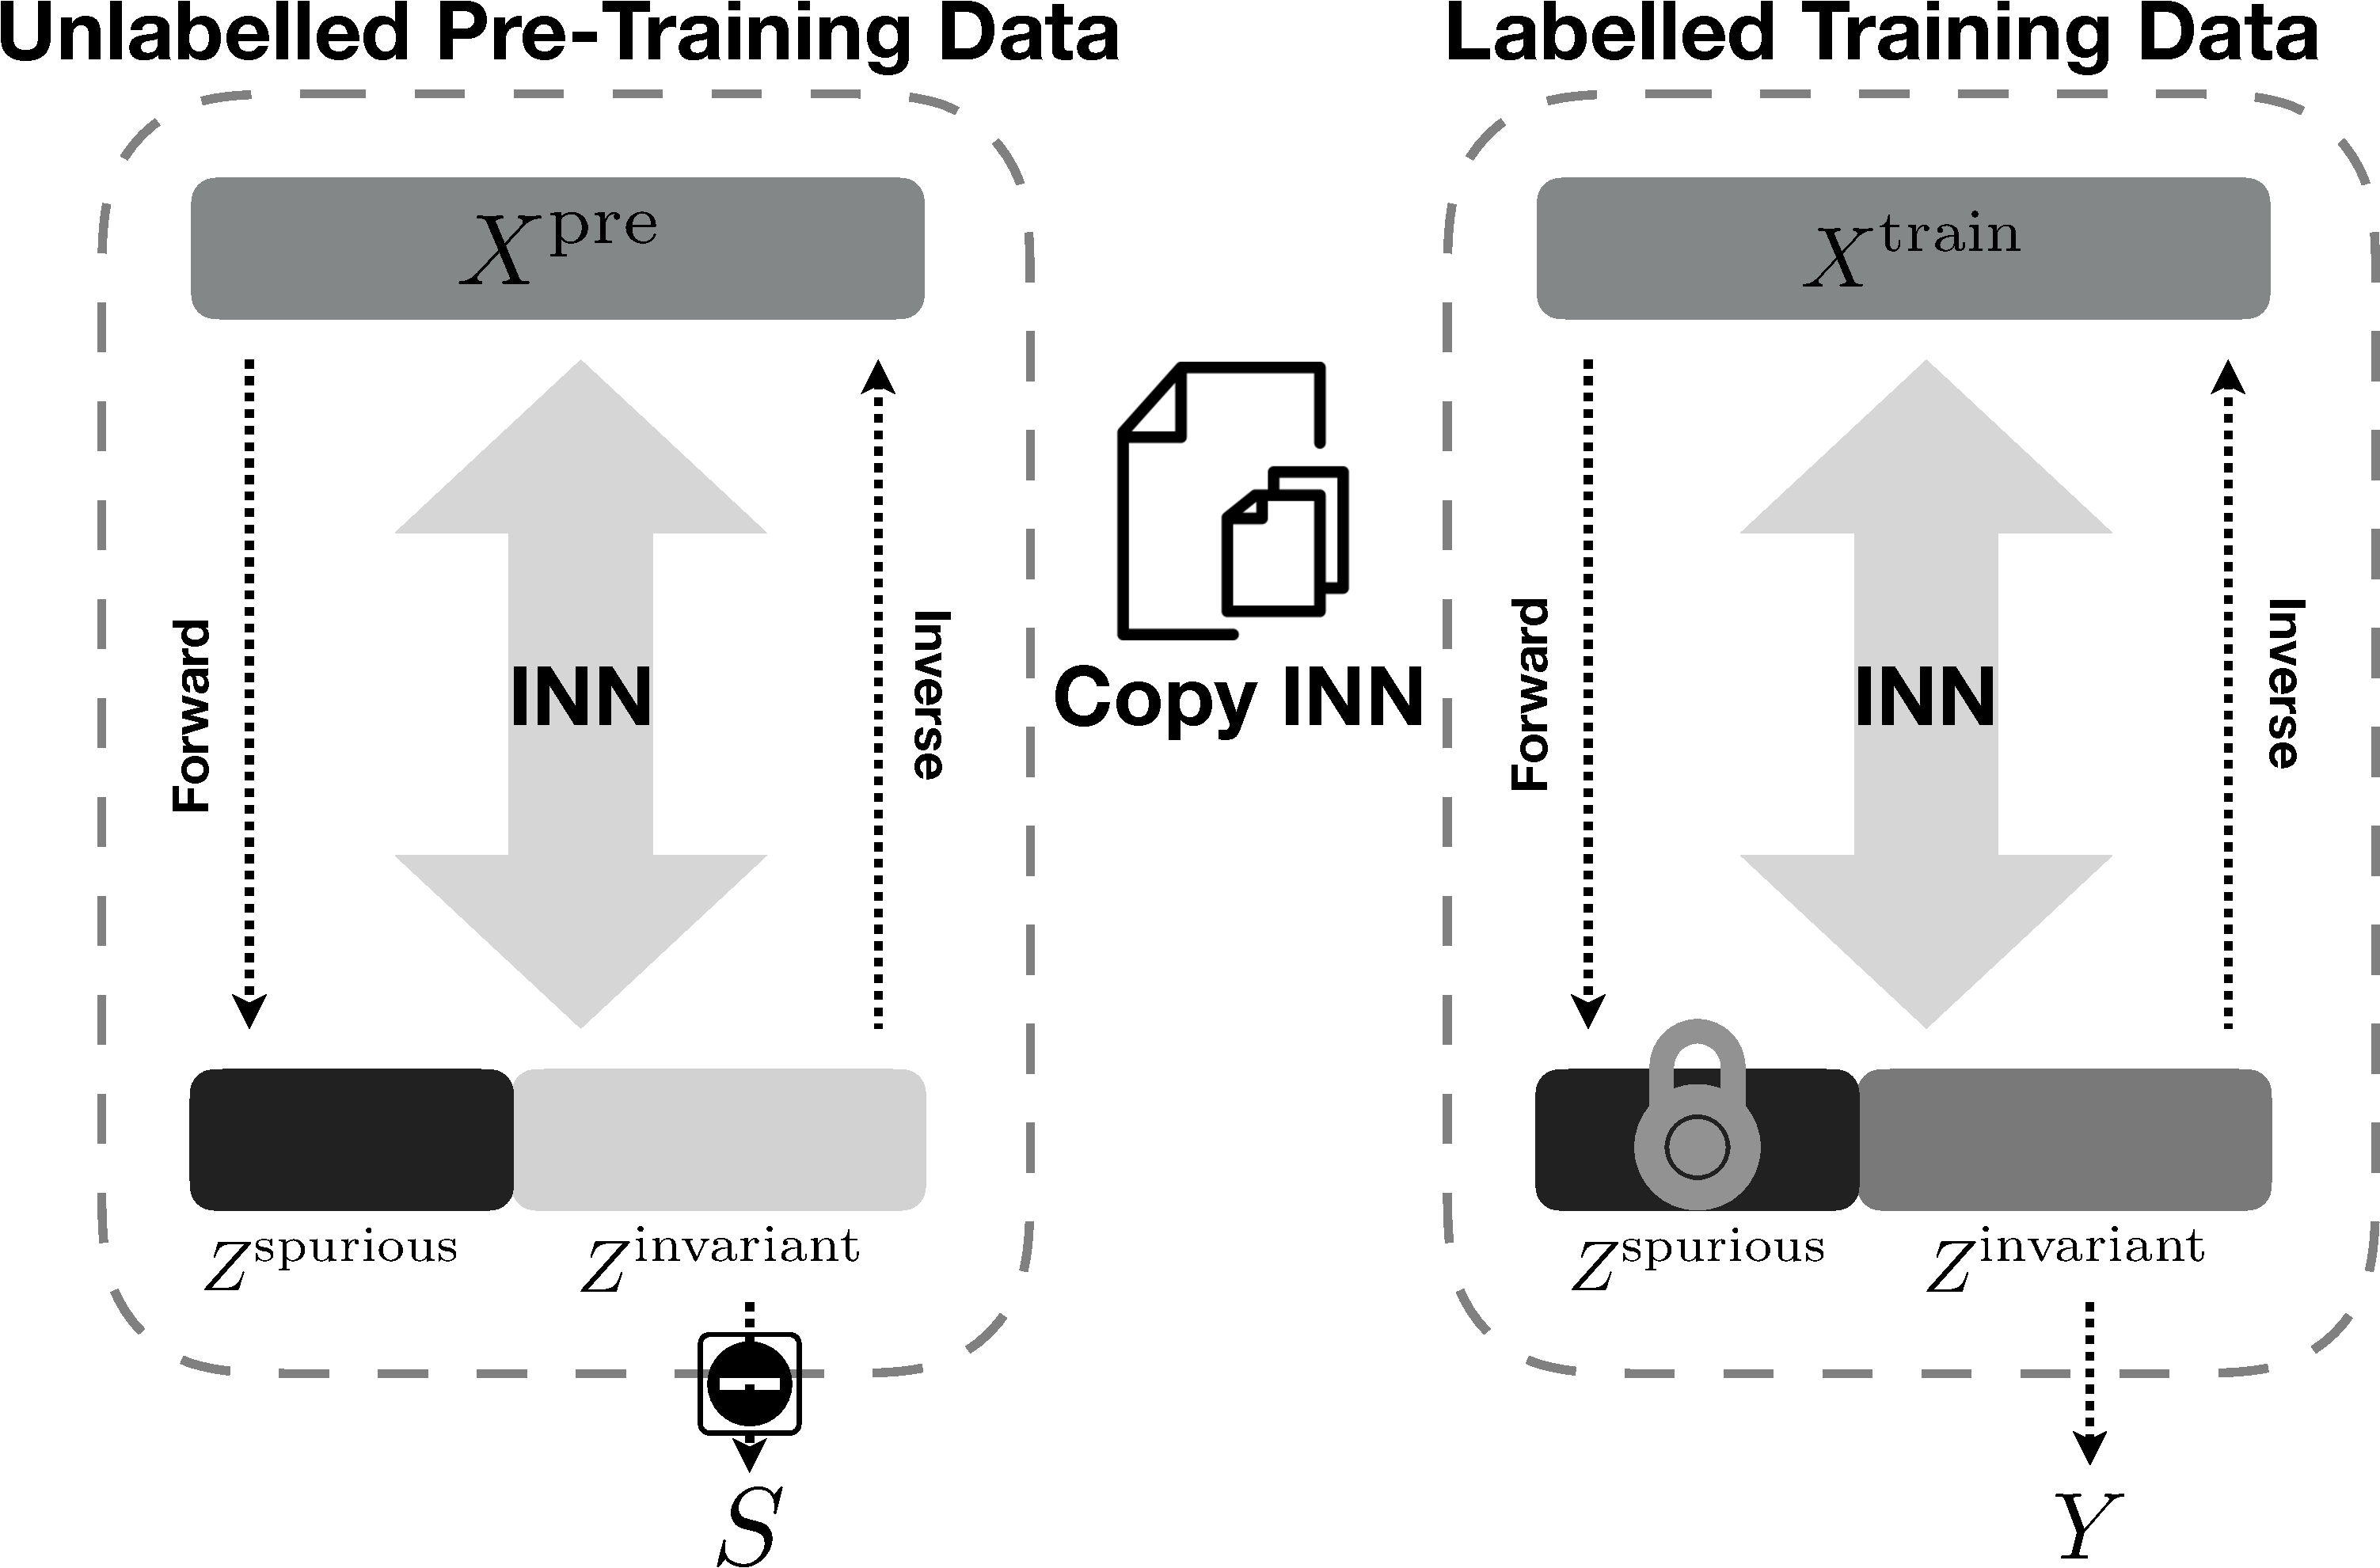
\includegraphics[width=0.4\textwidth]{./Figures/diagram.pdf}
%     \caption{Training procedure using the cFlow model for illustrative purposes.}%
%     \label{fig:training_diagram}
% \end{figure}
\begin{figure*}[tb]
    \centering
    \hfill
    \subfloat[cFlow model.]{%
        \scalebox{0.33}{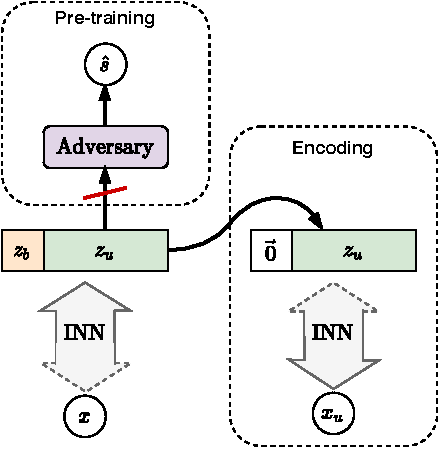
\includegraphics[width=\textwidth]{./Figures/inn_diagram_u.pdf}}%
        \label{fig:inn_diagram}
    }
    \hfill
    \subfloat[cVAE model.]{%
        \scalebox{0.4}{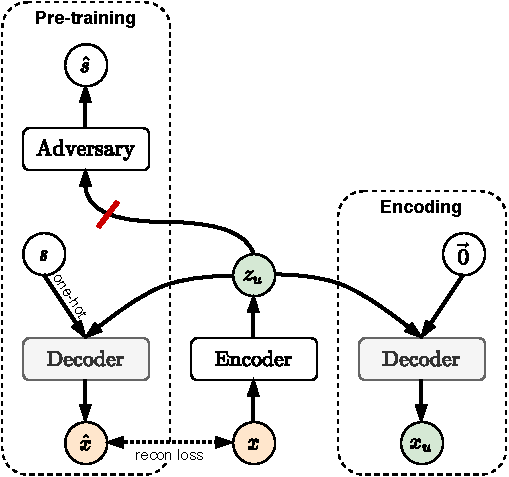
\includegraphics[width=\textwidth]{./Figures/cvae_diagram_u.pdf}}%
        \label{fig:cvae_diagram}
    }
    \hfill
    \caption{
        Training procedure for our models. $x$: input, $s$: sensitive attribute, $z_u$: de-biased representation, $x_u$: de-biased version of the input in the data domain.
        The red bar indicates a gradient reversal layer, and $\stackrel{\rightarrow}{0}$ the null-sampling operation.
    }%
    \label{fig:model-diagrams}
\end{figure*}

\subsection{Problem Statement} % HEADING IS JUST TO HELP ORGANIZE THOUGHTS, WILL BE DELETED LATER
\noindent We assume we are given inputs $\bm{x} \in \mathcal{X}$ and corresponding labels $y \in \mathcal{Y}$.
Furthermore, there is some spurious variable $s \in \mathcal{S}$ associated with each input $\bm{x}$ which we do \emph{not} want to predict. 
Let $X$, $S$ and $Y$ be random variables that take on the values $\bm{x}$, $s$ and $y$, respectively.
The fact that both $y$ and $s$ are predictive of $\bm{x}$ implies that $\mathcal{I}(X;Y), \mathcal{I}(X;S) > 0$, where $\mathcal{I}(\cdot ;\cdot)$ is the mutual information.
Note, however, that the conditional entropy is non-zero: $H(S|X) \neq 0$, i.e., $S$ is not completely determined by $X$.

%The difficulty emerges in the construction of the fully-supervised training dataset in which correspondence between $S$ and $Y$ is exaggerated compared to the test set.
The difficulty of this setup emerges in the training set: there is a close correspondence between $S$ and $Y$, such that for a model that sees the data through the lens of the loss function, the two are indistinguishable.
Furthermore, we assume that this is \emph{not} the case in the test set, meaning the model cannot rely on shortcuts provided by $S$ if it is to generalise from the training set.

We call this scenario where we only have access to the labels of a biasedly-sampled subpopulation
an \emph{aggravated fairness problem}.
These are not uncommon in the real-world.
For instance, in long-feedback systems such as mortgage-approval where the demographics of the subpopulation with observed outcomes is \emph{not} representative of the subpopulation on which the model has been deployed. 
In this case, $s$ has the potential to act as a false (or \emph{spurious}) indicator of the class label and
training a model with such a dataset would limit generalisability.
Let $(X^\mathit{tr}, S^\mathit{tr}, Y^\mathit{tr})$ then be the random variables sampled for the training set
and $(X^\mathit{te}, S^\mathit{te}, Y^\mathit{te})$ be the random variables for the test set.
The training and test sets thus induce the following inequality for their mutual information:
$\mathcal{I}(S^\mathit{tr}; Y^\mathit{tr}) \gg \mathcal{I}(S^\mathit{te}; Y^\mathit{te}) \approx 0$.

% \subsection{In an Ideal World} % HEADING IS JUST TO HELP ORGANIZE THOUGHTS, WILL BE DELETED LATER
Our goal is to learn a representation $\bm{z}_u$ that is independent of $s$ and transferable between downstream tasks.
Complementary to $\bm{z}_u$, we refer to some abstract component of the model that absorbs the unwanted information related to $s$ as $\mathcal{B}$, the realisation of which we define with respect to each of the two models to be described.
%To satisfy this objective, we introduce an additional regularisation term
%that can be viewed from an information-theoretic perspective as minimising the mutual information between the random variables:
The requirement for $\bm{z}_u$ can be expressed via mutual information:
\begin{align}
  I(\bm{z}_u;s) \overset{!}{=} 0~.
  \label{eq:migoal}
\end{align}
However, for the representation to be useful, we need to capture as much relevant information in the data as possible.
Thus, the combined objective function:
\begin{align}
  \min_{\theta} \mathbb{E}_{x \sim X}[-\log p_\theta(\bm{x})] + \lambda I(f_\theta(x);s)
  \label{eq:objectivetheory}
\end{align}
where $\theta$ refers to the trainable parameters of our model $f_\theta$ and $p_\theta(\bm{x})$ is the likelihood it assigns to the data.

We optimise this loss in an adversarial fashion by playing a min-max game, in which our encoder acts as the generative component.
The adversary is an auxiliary classifier $g$, which receives $\bm{z}_u$ as input and attempts to predict the spurious variable $s$.
We denote the parameters of the adversary as $\phi$;
for the parameters of the encoder we use $\theta$, as before.
The objective from~\eqref{eq:objectivetheory} is then% realised as
\begin{align}
  \min_{\theta\in\Theta} \max_{\phi\in\Phi} \mathbb{E}_{x \sim X}[\log p_\theta(x) -\lambda\mathcal{L}_c(g_\phi(f_\theta(x))); s)]
  \label{eq:objectivepractical}
\end{align}
where $\mathcal{L}_c$ is the cross-entropy between the predictions for $s$ and the provided labels.
In practice, this adversarial term is realised with a gradient reversal layer (GRL) \citep{ganin2016domain} between $\bm{z}_u$ and $g$ as is common in adversarial approaches~\citep{edwards2016censoring}.
% to fair representation learning

\subsection{The Disentanglement Dilemma} % HEADING IS JUST TO HELP ORGANIZE THOUGHTS, WILL BE DELETED LATER
The objective in~\eqref{eq:objectivepractical} balances the two desiderata: predicting $y$ and being invariant to $s$.
However, in the training set $(X^\mathit{tr}, S^\mathit{tr}, Y^\mathit{tr})$,
$y$ and $s$ are so strongly correlated that removing information about $s$ inevitably removes information about $y$.
This strong correlation makes existing methods fail under this setting.
% However, this objective is complicated by the desideratum that $\bm{z}_u$ remain predictive of $y$,
% which precludes us from directly training on the target-labelled dataset $(X^\mathit{tr}, S^\mathit{tr}, Y^\mathit{tr})$,
%where $y$ and $s$ are so strongly correlated that removing information about $s$ inevitably removes information about $y$.
%We therefore need
In order to even define the right learning goal,
we require another source of information that allows us to disentangle $s$ and $y$.
For this, we assume the existence of another set of samples that follow a similar distribution to the test set,
but whilst the sensitive attribute is available, the class labels are not.
In reality, this is not an unreasonable assumption,
as, while properly annotated data is scarce, unlabelled data can be obtained in abundance (with demographic information from census data, electoral rolls, etc.).
Previous work has also considered treated ``unlabelled data'' as still having $s$ labels~\citep{wick2019unlocking}.
We are restricted only in the sense that the spurious correlations we want to sever are indicated in the features.
We call this the \emph{representative set}, consisting of $X^\mathit{rep}$ and $S^\mathit{rep}$.
It fulfils $\mathcal{I}(S^\mathit{rep}; Y^\mathit{rep}) \approx 0$
(or rather, it would, if the class labels $Y^\mathit{rep}$ were available).
%{\color{red} justify the existence of such a dataset}

We now summarise the training procedure; an outline for the invertible network model (cFlow) can be seen in Fig.~\ref{fig:inn_diagram}.
First, the encoder network $f$ is trained on ($X^\mathit{rep}, S^\mathit{rep}$), during the first phase.
The trained network is then used to encode the training set,
taking in $\bm{x}$ and producing the representation, $\bm{z}_u$, decorrelated from the spurious variable.
The encoded dataset can then be used to train any off-the-shelf classifier safely, with information about the spurious variable having been absorbed by some auxiliary component $\mathcal{B}$.
In the case of the conditional VAE (cVAE) model,
$\mathcal{B}$ takes the form of the decoder subnetwork, which reconstructs the data conditional on a one-hot encoding of $s$,
while for the invertible network $\mathcal{B}$ is realised as a partition of the feature map $\bm{z}$
(such that $\bm{z} = [\bm{z}_u, \bm{z}_b]$), given the bijective constraint.
Thus, the classifier cannot take the shortcut of learning $s$ and instead must learn how to predict $y$ directly.
Obtaining the $s$-invariant representations, $\bm{x}_u$, in the data domain
is simply a matter of replacing the $\mathcal{B}$ component of the decoder's input for the cVAE,
and $\bm{z}_b$ for cFlow, with a zero vector of equivalent size.
We refer to this procedure used to generate $\bm{x}_u$ as \emph{null-sampling} (here, with respect to $\bm{z}_b)$.

% This That said, we do wish to draw a distinction between null-sampling and the annihilation operation featured in .
Null-sampling resembles the \emph{annihilation} operation described in \citet{xiao2017dna}, however we note that the two serve very different roles.  Whereas the annihilation operation serves as a regulariser to prevent trivial solutions (similar to \cite{jaiswal2018unsupervised}), null-sampling is used to generate the invariant representations post-training.

\subsection{Conditional Decoding}%
\label{conddec}
\noindent We first describe a VAE-based model similar to that proposed in~\citet{madras2018learning}, before highlighting some of its shortcomings that motivate the choice of an invertible representation learner.

The model takes the form of a class conditional $\beta$-VAE \citep{higgins2017beta}, in which the decoder is conditioned on the spurious attribute.
We use $\theta_{enc}, \theta_{dec} \in \theta$ to denote the parameters of the encoder and decoder sub-networks, respectively.
Concretely, the encoder component performs the mapping $x \rightarrow{\bm{z}_u}$, while $\mathcal{B}$ is instantiated as the decoder,
$\mathcal{B} \coloneqq p_{\theta_{dec}}(x|z_u, s)$, which takes in a concatenation of the learned non-spurious latent vector $\bm{z}_u$ and a one-hot encoding of the spurious label $s$ to produce a reconstruction of the input $\hat{x}$.
Conditioning on a one-hot encoding of $s$, rather than a single value, as done in \citet{madras2018learning} is the key to visualising invariant representations in the data domain.
If $\mathcal{I}(z_u; s)$ is properly minimised, the decoder can only derive its information about $s$ from the label, thereby freeing up $\bm{z}_u$ from encoding the unwanted information while still allowing for reconstruction of the input.
Thus, by feeding a zero-vector to the decoder we achieve $\hat{x} \perp s$.
The full learning objective for the cVAE is given as
\begin{align}
\begin{split}
    \mathcal{L}_{\mathrm{cVAE}} =& \mathbb{E}_{q_{\theta_{enc}}(z_u, b|x)}[\log p_{\theta_{dec}}(x|z, b) - \log p_{\theta_{dec}}(s|z_u)] \\ 
    &- \beta D_{KL}(q_{\theta_{enc}}(z_u |x) \| p(z_u))
\end{split}
\end{align}
where $\beta$ is a hyperparameter that determines the trade-off between reconstruction accuracy and independence constraints,
and $p(\bm{z}_u)$ is the prior imposed on the variational posterior.
For all our experiments, $p(\bm{z}_u)$ is realised as an Isotropic Gaussian.
Fig.~\ref{fig:cvae_diagram} summarises the procedure as a diagram.

While we show this setup can indeed work for simple problems, as~\citet{madras2018learning} before us have, we show that it lacks scalability due to disagreement between the components of the loss.
Since information about $s$ is only available to the decoder as a binary encoding,
if the relationship between $s$ and $x$ is highly non-linear and cannot be summarised by a simple on/off mechanism, as is the case if $s$ is an attribute such as gender,
off-loading information to the decoder by conditioning is no longer possible. As a result, $\bm{z}_u$ is forced to carry information about $s$ in order to minimise the reconstruction error. 

The obvious solution to this is to allow the encoder to store information about $s$ in a partition of the latent space as in  \citet{creager2019flexibly}.  However, we question whether an autoencoder is the best choice for this setup, with the view that an invertible model is the better tool for the task. Using an invertible model has several guarantees, namely complete information-preservation and freedom from a reconstruction loss, the importance of which we elaborate on below.

\subsection{Conditional Flow}\label{cflow}
\paragraph{Invertible Neural Networks.}
Invertible neural networks are a class of neural network architecture characterised by a bijective mapping between their inputs and output \citep{Dinh2014}. The transformations are designed such that their inverses and Jacobians are efficiently computable.
These flow-based models permit \emph{exact} likelihood estimation \citep{normflows2015} through the warping of a base density with a series of invertible transformations and computing the resulting, highly multi-modal, but still normalised, density, using the change of variable theorem:
% Flow-GAN \cite{grover2018flowgan} combines the \emph{exact} log-likelihood estimation of the invertible network with the adversarial training of a GAN.
\begin{align}
\begin{split}
  \log p(x) &= \log p(z) + 
   \sum \log \left| \det\left( \frac{\diff h_i}{ h_{i-1}}\right) \right|, %\\
  \quad p(z) = \mathcal{N}(z; 0, \mathbb{I})
  \label{eq:changeofvariables}
\end{split}
\end{align}
where $h_i$ refers to the outputs of the layers of the network and $p(z)$ is the base density, specifically an Isotropic Gaussian in our case.
Training of the invertible neural network is then reduced to maximising $\log p(x)$ over the training set,
i.e.\ maximising the probability the network assigns to samples in the training set.

% The requirement of analytic invertibility and Jacobians demands the use of a specialised subset of neural network layers, but the repertoire of practical invertible transformations has grown steadily over recent years, of which describe only the few we draw upon.

% \paragraph{Coupling layers}. Dinh et al. \cite{Dinh2014} introduced a simple yet powerful invertible transformation in the form of coupling layers. Ease of invertibility is achieved by updating only half of the input vector with a function that itself is trivially invertible but that is at the same time parameterised by a arbitrarily complex operation not subject to the invertibility constraint (e.g. a multi-layer neural network).
% Concretely, the vector $\bm{u}$ is split into two evenly sized vectors: $\bm{u} = [\bm{u}_1, \bm{u}_2]$.
% The output of the coupling layer is then a concatenation of vectors $\bm{v}_1$ and $\bm{v}_2$,
% where $\bm{v}_1 = s \cdot \bm{u}_1 + t$ and $\bm{v}_2 = \bm{u}_2$, with the affine parameters $s$ and $t$ generated by a non-invertible function of $\bm{u}_2$.

% \paragraph{1x1 Convolutions}. Kingma and Dhariwal \cite{KinDha18} introduced invertible 1x1 convolution as a generalised permutation operation and show that determinant can be computed efficiently using an LU decomposition of the weights.

% \paragraph{Spatial downsampling.} To downsample the spatial dimensions and promote mixing between the variables, \cite{Dinh2014} first mask the input with a checkerboard pattern before reshaping (transforming a $c \times h\times w$ tensor into a $4c \times \frac{1}{2} h\times \frac{1}{2}w$). Each "level" of the network is demarcated by a downsampling operation.

\paragraph{The Benefits of Bijectivity.}
Using an invertible network to generate our encoding, $\bm{z}_u$, carries a number of advantages over other approaches.
Ordinarily, the main benefit of flow-based models is that they permit exact density estimation. 
However, since we are not interested in sampling from the model's distribution, in our case the likelihood term serves as a regulariser, as it does for  \citet{JacSmeOya18}. 
Critically, this forces the mean of each latent dimension to zero enabling null-sampling. 
The invertible property of the network guarantees the preservation of all information relevant to $y$ which is independent of $s$, regardless of how it is allocated in the output space.
Secondly, we conjecture that the encodings are more robust to out-of-distribution data.
Whereas an autoencoder could map a previously seen input and a previously unseen input to the same representation,
an invertible network sidesteps this due to the network's bijective property, ensuring all relevant information is stored somewhere. This opens up the possibility of transfer learning between datasets with a similar manifestation of $s$, as we demonstrate in the Appendix~\ref{sec:transfer-learning}.

Under our framework, the invertible network $f$ maps the inputs $\bm{x}$ to a representation $\bm{z}_u$:
$f(\bm{x}) = \bm{z}$.
We interpret the embedding $\bm{z}$ as being the concatenation of two smaller embeddings: $\bm{z} = [\bm{z}_u, \bm{z}_b]$.
The dimensionality of $\bm{z}_b$, and $\bm{z}_u$, by complement, is a free parameter (see section~\ref{sec:optimisation-details} for tuning strategies).
As $f$ is invertible, $\bm{x}$ can be recovered like so:
\begin{align}
  \bm{x} = f^{-1}([\bm{z}_u, \bm{z}_b])
  \label{eq:zreconstruct}
\end{align}
where $\bm{z}_b$ is required for equality of the output dimension and input dimension to satisfy the bijectivity of the network -- we cannot output $\bm{z}_u$ alone, but have to output $\bm{z}_b$ as well. In order to generate the pre-image of $\bm{z}_u$, we perform null-sampling with respect to $\bm{z}_b$ by zeroing-out the elements of $\bm{z}_b$ (such that $\bm{x}_{u} = f^{-1}([\bm{z}_{u}, \stackrel{\rightarrow}{0}])$), i.e. setting them to the mean of the prior density, $\mathcal{N}(z;0, I)$.

How can we be sure that $\bm{z}_u$ contains enough information about $y$?
The importance of the invertible architecture bears out from this consideration. %, as the bijectivity of the network guarantees preservation of all information about the input. %
% The existence of the inverse, $f^{-1}$,  p $x$ from $z$ because $f^{-1}$ exists and can do just that.
As long as $\bm{z}_b$ does not contain the information about $y$, $\bm{z}_u$ necessarily must.
We can raise or lower the information capacity of $\bm{z}_b$ by adjusting its size;
this should be set to the smallest size sufficient to capture all information about $s$, so as not to sacrifice class-relevant information.
Section~\ref{sec:additional-results} explores the effects of the size further.

% Eq~\eqref{eq:zreconstruct} defines how to obtain $\bm{x}$.
% In order to generate the pre-image of $\bm{z}_u$, we perform null-sampling with respect to $\bm{z}_b$ by zeroing-out its elements -- i.e. setting them to the mean of the prior density imposed on $\bm{z}$, $\mathcal{N}(z;0, I)$ -- by the operation, $\bm{x}_{u} = f^{-1}([\bm{z}_{u}, \stackrel{\rightarrow}{0}])$.

% \paragraph{Tuning the Partition Sizes.}

% \paragraph{The Pitfalls of Adversarial Training.}

% \paragraph{Preprocessing}.
% Heuristically, we found that preprocessing the data with an autoencoder stabilises and accelerates training of the cFlow model. The autoencoder was pretrained on the pretraining set solely to minimise reconstruction loss and its weights frozen at the time of the INN's training. While this means the INN is not truly lossless with respect to the uncompressed data, its bijectivity is leveraged to ensure semantically-relevant information is not discarded during the pre-training phase, which is still applicable since the autoencoder is not trained jointly with the INN to maximise the adversarial loss. Since the autoencoder is optimised for compression, information about both the spurious and non-spurious attributes is captured impartially in its encoding.

%%%%%%%%% Experiments
%
\section{Experiments}
%
\noindent
%
We present experiments to demonstrate that the null-sampled representations are in fact invariant
to $s$ while still allowing a classifier to predict $y$ from them. 
%
We run our \ac{cVAE} and \ac{cFlow} models on the coloured MNIST (cMNIST) and CelebA dataset, which
we artificially bias, first describing the sampling procedure we follow to do so for non-synthetic
datasets. 
%
As baselines we have the model of~\citet{kim2019learning} (Ln2L) and the same \ac{CNN} used to
evaluate the \ac{cFlow} and \ac{cVAE} models but with the unmodified images as input (\acs{CNN}). 
%
For the \ac{cFlow} model we adopt a Glow-like architecture~\citep{KinDha18}, while both
sub-networks of the \ac{cVAE} model comprise gated convolutions~\citep{van2016conditional}, where
the encoding size is \(256\). 
%
For cMNIST, we construct the Ln2L baseline according to its original description, for CelebA, we
treat it as an augmentation of the baseline \ac{CNN}'s objective function.
%More
Detailed information regarding model architectures can be found in \S\ref{sec:architectures} and
\S\ref{sec:nifr-optimisation-details}.
%
\footnote{
    %
    Code can be found at \url{https://github.com/wearepal/nifr}.
    %
}
%
\begin{figure}[tb]
    \centering
    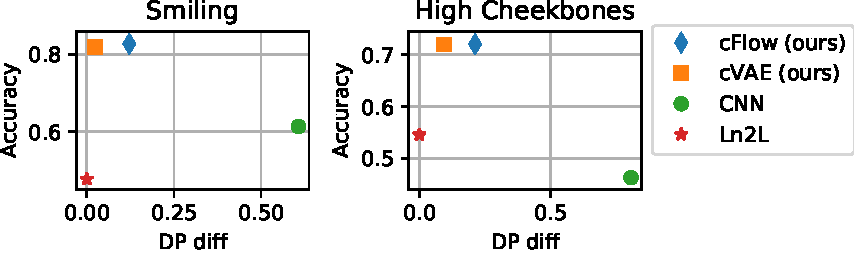
\includegraphics[width=0.7\textwidth]{nifr/Figures/nosinn_celeba.pdf}
    \caption{
        Performance of our model for different targets (mixing factor $\eta=0$).
        Left: \emph{Smiling} as target, right: \emph{high cheekbones}.
        \emph{DP diff} measures fairness with respect to demographic parity.
        A perfectly fair model has a \emph{DP diff} of 0.
    }%
    \label{fig:celeba-targets}
\end{figure}

\begin{figure}[tb]
    \centering
    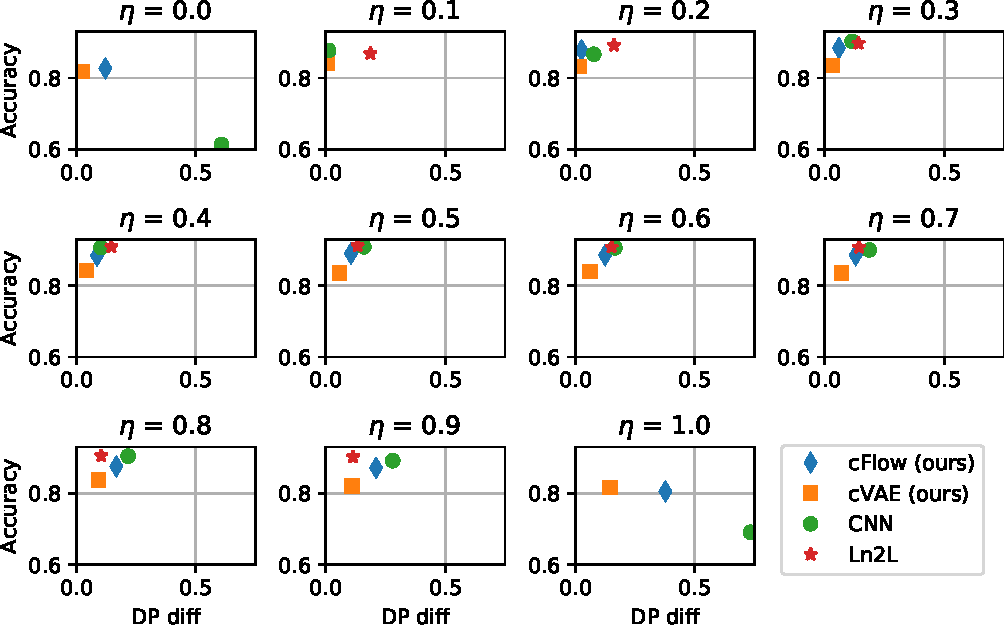
\includegraphics[width=0.85\textwidth]{nifr/Figures/nosinn_celeba_multiplot_all_landscape_Smiling.pdf}
    \caption{
        %
        Performance of our model for the target ``smiling'' for different mixing factors $\eta$.
        %
        \emph{DP diff} measures fairness with respect to demographic parity.
        %
        A perfectly fair model has a \emph{DP diff} of 0, thus the closer to top-left the better it
        is in terms of we accuracy-fairness trade-off.
        %
        Only values $\eta=0$ and $\eta=1$ correspond to the scenario of a strongly biased training
        set.
        %
        The results for $0.1\leq \eta\leq 0.9$ are to confirm that our model does not harm
        performance for non-biased training sets.
    }%
    \label{fig:celeba-multiplot}
\end{figure}
%
\subsection{Synthesising Dataset Bias}
%
For our experiments, we require a training set that exhibits a strong spurious correlation,
together with a test set that does not.
%
For cMNIST, this is easily satisfied as we have complete control over the data generation process.
%
For CelebA and  UCI Adult, on the other hand, we have to generate the split from the existing data.
%
To this end, we first set aside a randomly selected portion of the dataset from which to sample the
biased dataset.
%
The resulting portion is then split further into two parts: one in which \( (s=-1 \land y=-1) \lor
(s=+1 \land y=+1) \) holds true for all samples, call this part \( \mathcal{D}_{eq} \), and the
other part, call it \( \mathcal{D}_{opp} \), which contains the remaining samples.
%
To investigate the behaviour at different levels of correlation, we mix these two subsets according
to a mixing factor \( \eta \).
%
For $\eta \leq \tfrac{1}{2}$, we combine (all of) $\mathcal{D}_{eq}$ with a fraction of $2\eta$
from $\mathcal{D}_{opp}$.
%
For $\eta > \tfrac{1}{2}$, we combine (all of) $\mathcal{D}_{opp}$ and a fraction of $2(1 -\eta)$
from $\mathcal{D}_{eq}$.
%
Thus, for $\eta=0$, the biased dataset is just $\mathcal{D}_{eq}$, for $\eta=1$ it is just
$\mathcal{D}_{opp}$ and for $\eta=\tfrac{1}{2}$ the biased dataset is an ordinary subset of the
whole data. The test set is simply the data remaining from the initial split.
%
\subsection{Evaluation protocol}
%
We evaluate our results in terms of accuracy and fairness. A model that perfectly decouples its
predictions from $s$ will achieve near-uniform accuracy across all biasing-levels. 
%
For binary $s$/$y$ we quantify the fairness of a classifier's predictions using \emph{demographic
parity} (DP): the  absolute difference in the probability  of a positive prediction for each
sensitive group.

\begin{figure}[tb]
    \centering
    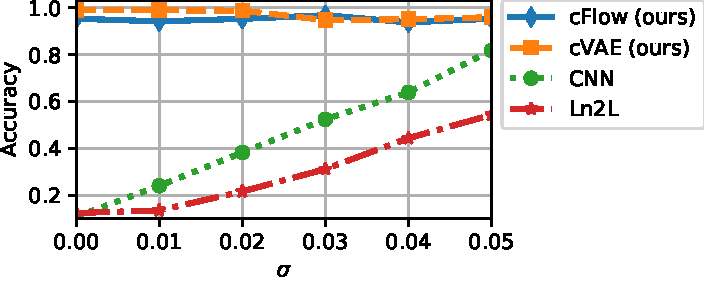
\includegraphics[width=0.7\textwidth]{nifr/Figures/cmnist_new_no_hgr.pdf}
    \caption{
        Accuracy of our approach in comparison with other baseline models on the cMNIST dataset,
        for different standard deviations ($\sigma$) for the colour sampling.
    }%
    \label{fig:cmnist_chart}
\end{figure}

\begin{figure*}[!htb]
    \centering
    \subfloat[Samples from the cMNIST training set, $\sigma=0$.]{%
        \scalebox{0.3}{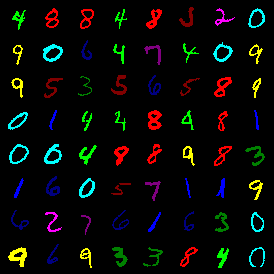
\includegraphics[width=\textwidth]{nifr/Images/cmnist/cflow_original_task_x_scale_0.png}}%
        \label{fig:cflow_cmnist_task_train}
    }
    \hfill
    \subfloat[$x_u$ null-samples from the \ac{cFlow} model.]{%
        \scalebox{0.3}{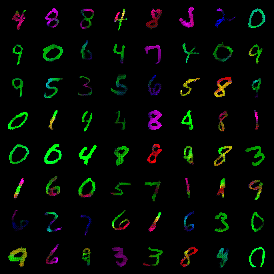
\includegraphics[width=\textwidth]{nifr/Images/cmnist/cflow_task_xy_scale_0.png}}%
        \label{fig:cflow_cmnist_y}
    }
    \hfill
    \subfloat[$x_b$ null-samples from the \ac{cFlow} model.]{%
        \scalebox{0.3}{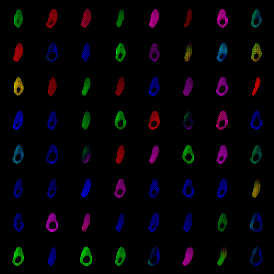
\includegraphics[width=\textwidth]{nifr/Images/cmnist/cflow_task_xs_scale_0.png}}%
        \label{fig:cflow_cmnist_s}
    }
    \caption{
        %
        Sample images from the coloured MNIST dataset problem with $10$ predefined mean colours.
        %
        (a): Images from the spuriously correlated subpopulation where colour is a reliable signal
        of the digit class-label.
        %
        (b-c): Results of running our approach realised with \ac{cFlow} on the cMNIST dataset.
        %
        The model learns to retain the shape of the digit while removing the relationship with
        colour.
        %
        A downstream classifier is now less prone to exploiting correlations between colour and the
        digit label class.
        %
    }\label{fig:cmnist}
\end{figure*}
%
\subsection{Experimental results}
%
We report the results from two image datasets. cMNIST, a synthetic dataset, is a good starting
point for evaluating our model due to the direct control we have over the biasing. 
%
CelebA, on the other hand, is a more practical and challenging example.
%
We also test our method on a tabular dataset, the Adult dataset.
%
\paragraph{cMNIST.}
%
The coloured MNIST (cMNIST) dataset is a variant of the MNIST dataset in which the digits are
coloured.
%
In the training set, the colours have a one-to-one correspondence with the digit class.
%
In the test set (and the representative set), colours are assigned randomly.
%
The colours are drawn from Gaussians with 10 different means.
%
We follow the colourisation procedure outlined by~\citet{kim2019learning}, with the mean colour
values selected so as to be maximally dispersed.
%
The full list of such values can be found in \S\ref{sec:color-details}.
%
We produce multiple variants of the cMNIST dataset corresponding to different standard deviations
$\sigma$ for the colour sampling: $\sigma \in \{0.00, 0.01, ..., 0.05 \}$.

For this specific dataset, we can establish an additional baseline by simply grey-scaling the
dataset which only leaves the luminosity as spurious information.
%
We also evaluate the model, with all the associated hyperparameters, from~\citet{kim2019learning}.
%
The only difference between the setups is the dataset creation, including the range of \(\sigma\)
values we consider.
%
Our versions of the dataset, on the whole, exhibit much stronger colour bias, to the point of the
mapping the digit's colour and class being bijective. 
%
Fig.~\ref{fig:cmnist_chart} shows that the model significantly underperforms even the na\"ive
baseline, aside from at \(\sigma = 0\), where they are at parity.
%
\corr{
%
Ln2L relies upon adversarial \ac{MI}-minimisation in the fashion of \citet{ganin2016domain}; we
conjecture that the sub-\ac{CNN} performance of Ln2L is consequent of the optimum of this objective
connoting invariance to both the digit and colour, as one may serve as an effective (with degree
scaling inversely with \(\sigma\)) for the other for both the classifier and the adversary, in
absence of partially-unlabelled data to decouple the attributes.
%
We would also expect invariance is also expected of the \ac{CNN} as a by-product of the excessive
variance to colour (that is to say, colour being a shortcut means that digit-information is
redundant, albeit -- importantly -- not deliberately excised) and the results indicate an
increasing noise-level alone more effectively breaks this than the aforementioned,
explicitly-enforced invariance (which is itself subject to noise, in addition with the predictive
streams) in tandem with it.
%
This degenerate behaviour of Ln2L may be attenuated with more judicious choice of pre-factor on
said \ac{MI}-minimisation term, though the problem hyperparameter selection for \ac{DG} problems is
challenging in its own right \citep{gulrajani2020search}; our method requires minimal consideration
in this respect due to non-conflicting objectives.
}
% CORRECTED: need more explanation of the figures here for me. Maybe can expand now you don't have
% page constraints. In particular comment on whey LN2L does so badly

Inspection of the null-samples shows that both the \ac{cVAE} and \ac{cFlow} model succeed in
removing almost all colour information, which is supported quantitatively by
Fig.~\ref{fig:cmnist_chart}, and qualitatively by Fig.~\ref{fig:cmnist}. 
%
While the \ac{cVAE} outperforms \ac{cFlow} marginally at low \(\sigma\) values, performance degrades
%rapidly
as this increases. 
%
This highlights the problems with the conditional decoder we anticipated in \S\ref{conddec}. 
%
The lower $\sigma$, and therefore the variation in sampled colour, is, the more reliably the $s$
label, corresponding to the mean of RGB distribution, encodes information about the colour. 
%
For higher $\sigma$ values, the sampled colours can deviate far from the mean and so the encoder
must incorporate information about $s$ into its representation if it is to minimise the
reconstruction loss. \ac{cFlow}, on the other hand, is consistent across $\sigma$ values.
%
\paragraph{CelebA.}
%
To evaluate the effectiveness of our framework on real-world image data we use the CelebA
dataset~\citep{liu2015faceattributes}, consisting of 202,599 celebrity images. 
%
These images are annotated with various binary physical  attributes, including ``gender'', ``hair
colour'', ``young'', etc., from which we select our sensitive and target attributes. 
%
The images are centre cropped and resized to $64\times64$, as is standard practice. 
%
For our experiments, we designate ``gender'' as the sensitive attribute, and ``smiling'' and ``high
cheekbones'' as target attributes. 
%
We chose gender as the sensitive attribute as it a common sensitive attribute in the fairness
literature. 
%
For the target attributes, we chose attributes that are harder to learn than gender and which do
not correlate too strongly with gender in the dataset (``wearing lipstick'' for example being an
attribute too closely correlated with gender).
%
The model is trained on the representative set (normal subset of CelebA) and is then used to encode
the artificially biased training set and the test set. The results for the most strongly biased
training set ($\eta=0$) can be found in Fig.~\ref{fig:celeba-targets}. Our method outperforms the
baselines in accuracy and fairness.

\begin{figure*}[tb]
  \centering
  \subfloat[Original images.]{%
      \scalebox{0.3}{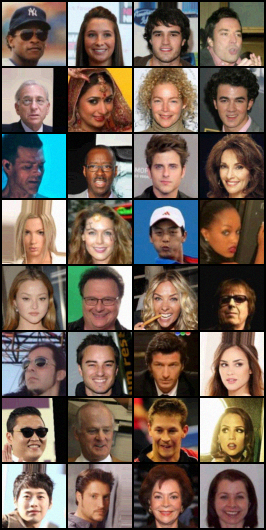
\includegraphics[width=\textwidth]{nifr/Images/celeba/train_original_x_2.png}}%
      \label{fig:cflow_celeba_original_x}
  }
  \hfill
  \subfloat[$\bm{x}_u$ null-samples from the cFlow model.]{%
      \scalebox{0.3}{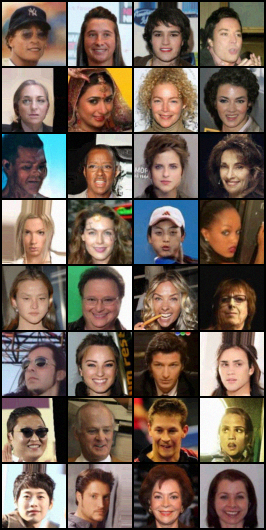
\includegraphics[width=\textwidth]{nifr/Images/celeba/train_reconstruction_y_2.png}}%
      \label{fig:cflow_celeba_recon_y}
  }
  \hfill
  \subfloat[$\bm{x}_b$ null-samples from the cFlow model.]{%
      \scalebox{0.3}{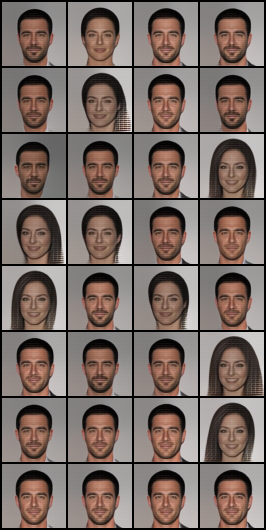
\includegraphics[width=\textwidth]{nifr/Images/celeba/train_reconstruction_s_2.png}}%
      \label{fig:cflow_celeba_recon_s}
  }
  \caption{
      CelebA null-samples learned by our \ac{cFlow} model, with gender as the sensitive attribute.
      %
      (a) The original, untransformed samples from the CelebA dataset
    %
      (b) Reconstructions using only information unrelated to $s$.
    %
      (c) Reconstruction using only information related to $\neg s$.
    %
      The model learns to disentangle gender from the non-gender related information.
      %
      Note that some attributes like skin tone seem to change along with gender due to the
      correlation between the attributes.
    %
      This is especially visible in images (1,1) and (3,2). Only because our representations are
      produced in the data-domain can we easily spot such instances of entanglement.
  }%
  \label{fig:celeba_cflow}
\end{figure*}
%
We also assess performance for different mixing factors ($\eta$) which correspond to varying
degrees of bias in the training set (see Fig.~\ref{fig:celeba-multiplot}).
%
This is to verify that the model does not \emph{harm} performance when there is not much bias in
the training set.
%
For these experiments, the model is trained once on the representative set and is then used to
encode different training sets.
%
The results show that for the intermediate values of $\eta$, our model incurs a small penalty in
terms of accuracy, but at the same time makes the results \emph{fairer} (corresponding to an
accuracy-fairness trade-off). 
%
Qualitative results can be found in Fig.~\ref{fig:celeba_cflow} (images from \ac{cVAE} can be found
in \S\ref{sec:qual-results-celeba}).

To show that our method can handle multinomial, as well as binary, sensitive attributes, we also
conduct experiments with $s=\textrm{hair colour}$ as a ternary attribute (``Blonde'', ``Black'',
``Brown''), excluding ``Red'' because of the paucity of samples and the noisiness of their labels.
%
The results for these experiments can be found in \S\ref{sec:additional-results}.

\begin{figure}[tb]
  \centering
  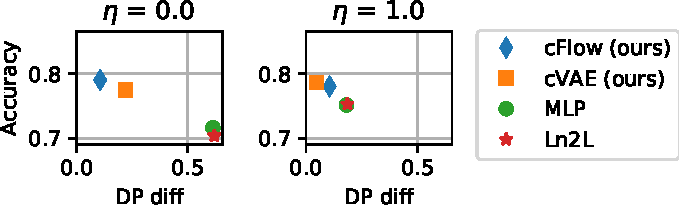
\includegraphics[width=0.6\textwidth]{nifr/Figures/nosinn_adult_multiplot_mini_diff.pdf}
  \caption{
      Results for the \textsc{Adult} dataset.
      The $x$-axis corresponds to the difference in positive rates.
      An ideal result would occupy the \textsc{top-left}.
  }%
  \label{fig:adult-chart}
\end{figure}
% \end{wrapfigure}

\paragraph{Results for the UCI Adult dataset.}
%
The UCI Adult dataset consists of census data and is commonly used to evaluate models focused on
\acl{AF}.
%
Following convention, we designate ``gender'' as the sensitive attribute $s$ and whether an
individual's salary is \$50,000 or greater as $y$.
%
We show the performance of our approach in comparison to baseline approaches in Fig.
\ref{fig:adult-chart}.
%
We evaluate the performance of all models for mixing factors ($\eta$) $0$ and $1$. 
%
Results shown in Fig. \ref{fig:adult-chart} show that we match or exceed the baseline.
%
In terms of fairness metrics, our approach generally outperforms the baseline models for both of
$\eta$.
%
Detailed results can be found in \S\ref{sec:additional-results}.

We also did experiments to show that the encoder transfers to other tasks. 
%
These transfer-learning experiments can be found in \S\ref{sec:transfer-learning}.


\section{Conclusion}\label{sec:nifr-conclusion}
%
We have proposed a general and straightforward framework for producing invariant representations,
under the assumption that a representative but partially-labelled \emph{representative} set is
available. 
%
Training consists of two stages: an encoder is first trained on the representative set to produce a
representation that is invariant to a designated spurious feature. 
%
This is then used as input for a downstream task-classifier, the training data for which might
exhibit extreme bias with respect to that feature. 
%
We train both a \acs{VAE}- and \acs{INN}-based model according to this procedure, and show that the
latter is particularly well-suited to this setting due to its losslessness. 
%
The design of the models allows for representations that are in the data domain and therefore
exhibit meaningful invariances. 
%
We characterise this for synthetic as well as real-world datasets for which we develop a method for
simulating sampling bias.
%


\section*{Acknowledgements}
This work was in part funded by the European Research Council 
under the ERC grant agreement no. 851538.
We are grateful to NVIDIA for donating GPUs.

%%%%%%%%% ICML 2021 EXAMPLE LATEX SUBMISSION FILE %%%%%%%%%%%%%%%%%

%\documentclass{article}

%% Optional math commands from https://github.com/goodfeli/dlbook_notation.
%%%%%% NEW MATH DEFINITIONS %%%%%

\usepackage{amsmath,amsfonts,bm}

% Mark sections of captions for referring to divisions of figures
\newcommand{\figleft}{{\em (Left)}}
\newcommand{\figcenter}{{\em (Center)}}
\newcommand{\figright}{{\em (Right)}}
\newcommand{\figtop}{{\em (Top)}}
\newcommand{\figbottom}{{\em (Bottom)}}
\newcommand{\captiona}{{\em (a)}}
\newcommand{\captionb}{{\em (b)}}
\newcommand{\captionc}{{\em (c)}}
\newcommand{\captiond}{{\em (d)}}

% Highlight a newly defined term
\newcommand{\newterm}[1]{{\bf #1}}


% Figure reference, lower-case.
\def\figref#1{figure~\ref{#1}}
% Figure reference, capital. For start of sentence
\def\Figref#1{Figure~\ref{#1}}
\def\twofigref#1#2{figures \ref{#1} and \ref{#2}}
\def\quadfigref#1#2#3#4{figures \ref{#1}, \ref{#2}, \ref{#3} and \ref{#4}}
% Section reference, lower-case.
\def\secref#1{section~\ref{#1}}
% Section reference, capital.
\def\Secref#1{Section~\ref{#1}}
% Reference to two sections.
\def\twosecrefs#1#2{sections \ref{#1} and \ref{#2}}
% Reference to three sections.
\def\secrefs#1#2#3{sections \ref{#1}, \ref{#2} and \ref{#3}}
% Appendix reference, lower-case.
\def\appref#1{appendix~\ref{#1}}
% Appendix reference, capital.
\def\Appref#1{Appendix~\ref{#1}}
% Reference to an equation, lower-case.
\def\eqref#1{equation~\ref{#1}}
% Reference to an equation, upper case
\def\Eqref#1{Equation~\ref{#1}}
% A raw reference to an equation---avoid using if possible
\def\plaineqref#1{\ref{#1}}
% Reference to a chapter, lower-case.
\def\chapref#1{chapter~\ref{#1}}
% Reference to a Chapter, upper case.
\def\Chapref#1{Chapter~\ref{#1}}
\def\twochaprefs#1#2{chapters \ref{#1} and \ref{#2}}
% Reference to a range of chapters
\def\rangechapref#1#2{chapters \ref{#1}--\ref{#2}}
% Reference to a range of chapters, upper case
\def\Rangechapref#1#2{Chapters \ref{#1}--\ref{#2}}
% Reference to an algorithm, lower-case.
\def\algref#1{algorithm~\ref{#1}}
% Reference to an algorithm, upper case.
\def\Algref#1{Algorithm~\ref{#1}}
\def\twoalgref#1#2{algorithms \ref{#1} and \ref{#2}}
\def\Twoalgref#1#2{Algorithms \ref{#1} and \ref{#2}}
% Reference to a part, lower case
\def\partref#1{part~\ref{#1}}
% Reference to a part, upper case
\def\Partref#1{Part~\ref{#1}}
\def\twopartref#1#2{parts \ref{#1} and \ref{#2}}

\def\ceil#1{\lceil #1 \rceil}
\def\floor#1{\lfloor #1 \rfloor}
\def\1{\bm{1}}
\newcommand{\train}{\mathcal{D}}
\newcommand{\valid}{\mathcal{D_{\mathrm{valid}}}}
\newcommand{\test}{\mathcal{D_{\mathrm{test}}}}

\def\eps{{\epsilon}}


% Random variables
\def\reta{{\textnormal{$\eta$}}}
\def\ra{{\textnormal{a}}}
\def\rb{{\textnormal{b}}}
\def\rc{{\textnormal{c}}}
\def\rd{{\textnormal{d}}}
\def\re{{\textnormal{e}}}
\def\rf{{\textnormal{f}}}
\def\rg{{\textnormal{g}}}
\def\rh{{\textnormal{h}}}
\def\ri{{\textnormal{i}}}
\def\rj{{\textnormal{j}}}
\def\rk{{\textnormal{k}}}
\def\rl{{\textnormal{l}}}
% rm is already a command, just don't name any random variables m
\def\rn{{\textnormal{n}}}
\def\ro{{\textnormal{o}}}
\def\rp{{\textnormal{p}}}
\def\rq{{\textnormal{q}}}
\def\rr{{\textnormal{r}}}
\def\rs{{\textnormal{s}}}
\def\rt{{\textnormal{t}}}
\def\ru{{\textnormal{u}}}
\def\rv{{\textnormal{v}}}
\def\rw{{\textnormal{w}}}
\def\rx{{\textnormal{x}}}
\def\ry{{\textnormal{y}}}
\def\rz{{\textnormal{z}}}

% Random vectors
\def\rvepsilon{{\mathbf{\epsilon}}}
\def\rvtheta{{\mathbf{\theta}}}
\def\rva{{\mathbf{a}}}
\def\rvb{{\mathbf{b}}}
\def\rvc{{\mathbf{c}}}
\def\rvd{{\mathbf{d}}}
\def\rve{{\mathbf{e}}}
\def\rvf{{\mathbf{f}}}
\def\rvg{{\mathbf{g}}}
\def\rvh{{\mathbf{h}}}
\def\rvu{{\mathbf{i}}}
\def\rvj{{\mathbf{j}}}
\def\rvk{{\mathbf{k}}}
\def\rvl{{\mathbf{l}}}
\def\rvm{{\mathbf{m}}}
\def\rvn{{\mathbf{n}}}
\def\rvo{{\mathbf{o}}}
\def\rvp{{\mathbf{p}}}
\def\rvq{{\mathbf{q}}}
\def\rvr{{\mathbf{r}}}
\def\rvs{{\mathbf{s}}}
\def\rvt{{\mathbf{t}}}
\def\rvu{{\mathbf{u}}}
\def\rvv{{\mathbf{v}}}
\def\rvw{{\mathbf{w}}}
\def\rvx{{\mathbf{x}}}
\def\rvy{{\mathbf{y}}}
\def\rvz{{\mathbf{z}}}

% Elements of random vectors
\def\erva{{\textnormal{a}}}
\def\ervb{{\textnormal{b}}}
\def\ervc{{\textnormal{c}}}
\def\ervd{{\textnormal{d}}}
\def\erve{{\textnormal{e}}}
\def\ervf{{\textnormal{f}}}
\def\ervg{{\textnormal{g}}}
\def\ervh{{\textnormal{h}}}
\def\ervi{{\textnormal{i}}}
\def\ervj{{\textnormal{j}}}
\def\ervk{{\textnormal{k}}}
\def\ervl{{\textnormal{l}}}
\def\ervm{{\textnormal{m}}}
\def\ervn{{\textnormal{n}}}
\def\ervo{{\textnormal{o}}}
\def\ervp{{\textnormal{p}}}
\def\ervq{{\textnormal{q}}}
\def\ervr{{\textnormal{r}}}
\def\ervs{{\textnormal{s}}}
\def\ervt{{\textnormal{t}}}
\def\ervu{{\textnormal{u}}}
\def\ervv{{\textnormal{v}}}
\def\ervw{{\textnormal{w}}}
\def\ervx{{\textnormal{x}}}
\def\ervy{{\textnormal{y}}}
\def\ervz{{\textnormal{z}}}

% Random matrices
\def\rmA{{\mathbf{A}}}
\def\rmB{{\mathbf{B}}}
\def\rmC{{\mathbf{C}}}
\def\rmD{{\mathbf{D}}}
\def\rmE{{\mathbf{E}}}
\def\rmF{{\mathbf{F}}}
\def\rmG{{\mathbf{G}}}
\def\rmH{{\mathbf{H}}}
\def\rmI{{\mathbf{I}}}
\def\rmJ{{\mathbf{J}}}
\def\rmK{{\mathbf{K}}}
\def\rmL{{\mathbf{L}}}
\def\rmM{{\mathbf{M}}}
\def\rmN{{\mathbf{N}}}
\def\rmO{{\mathbf{O}}}
\def\rmP{{\mathbf{P}}}
\def\rmQ{{\mathbf{Q}}}
\def\rmR{{\mathbf{R}}}
\def\rmS{{\mathbf{S}}}
\def\rmT{{\mathbf{T}}}
\def\rmU{{\mathbf{U}}}
\def\rmV{{\mathbf{V}}}
\def\rmW{{\mathbf{W}}}
\def\rmX{{\mathbf{X}}}
\def\rmY{{\mathbf{Y}}}
\def\rmZ{{\mathbf{Z}}}

% Elements of random matrices
\def\ermA{{\textnormal{A}}}
\def\ermB{{\textnormal{B}}}
\def\ermC{{\textnormal{C}}}
\def\ermD{{\textnormal{D}}}
\def\ermE{{\textnormal{E}}}
\def\ermF{{\textnormal{F}}}
\def\ermG{{\textnormal{G}}}
\def\ermH{{\textnormal{H}}}
\def\ermI{{\textnormal{I}}}
\def\ermJ{{\textnormal{J}}}
\def\ermK{{\textnormal{K}}}
\def\ermL{{\textnormal{L}}}
\def\ermM{{\textnormal{M}}}
\def\ermN{{\textnormal{N}}}
\def\ermO{{\textnormal{O}}}
\def\ermP{{\textnormal{P}}}
\def\ermQ{{\textnormal{Q}}}
\def\ermR{{\textnormal{R}}}
\def\ermS{{\textnormal{S}}}
\def\ermT{{\textnormal{T}}}
\def\ermU{{\textnormal{U}}}
\def\ermV{{\textnormal{V}}}
\def\ermW{{\textnormal{W}}}
\def\ermX{{\textnormal{X}}}
\def\ermY{{\textnormal{Y}}}
\def\ermZ{{\textnormal{Z}}}

% Vectors
\def\vzero{{\bm{0}}}
\def\vone{{\bm{1}}}
\def\vmu{{\bm{\mu}}}
\def\vtheta{{\bm{\theta}}}
\def\va{{\bm{a}}}
\def\vb{{\bm{b}}}
\def\vc{{\bm{c}}}
\def\vd{{\bm{d}}}
\def\ve{{\bm{e}}}
\def\vf{{\bm{f}}}
\def\vg{{\bm{g}}}
\def\vh{{\bm{h}}}
\def\vi{{\bm{i}}}
\def\vj{{\bm{j}}}
\def\vk{{\bm{k}}}
\def\vl{{\bm{l}}}
\def\vm{{\bm{m}}}
\def\vn{{\bm{n}}}
\def\vo{{\bm{o}}}
\def\vp{{\bm{p}}}
\def\vq{{\bm{q}}}
\def\vr{{\bm{r}}}
\def\vs{{\bm{s}}}
\def\vt{{\bm{t}}}
\def\vu{{\bm{u}}}
\def\vv{{\bm{v}}}
\def\vw{{\bm{w}}}
\def\vx{{\bm{x}}}
\def\vy{{\bm{y}}}
\def\vz{{\bm{z}}}

% Elements of vectors
\def\evalpha{{\alpha}}
\def\evbeta{{\beta}}
\def\evepsilon{{\epsilon}}
\def\evlambda{{\lambda}}
\def\evomega{{\omega}}
\def\evmu{{\mu}}
\def\evpsi{{\psi}}
\def\evsigma{{\sigma}}
\def\evtheta{{\theta}}
\def\eva{{a}}
\def\evb{{b}}
\def\evc{{c}}
\def\evd{{d}}
\def\eve{{e}}
\def\evf{{f}}
\def\evg{{g}}
\def\evh{{h}}
\def\evi{{i}}
\def\evj{{j}}
\def\evk{{k}}
\def\evl{{l}}
\def\evm{{m}}
\def\evn{{n}}
\def\evo{{o}}
\def\evp{{p}}
\def\evq{{q}}
\def\evr{{r}}
\def\evs{{s}}
\def\evt{{t}}
\def\evu{{u}}
\def\evv{{v}}
\def\evw{{w}}
\def\evx{{x}}
\def\evy{{y}}
\def\evz{{z}}

% Matrix
\def\mA{{\bm{A}}}
\def\mB{{\bm{B}}}
\def\mC{{\bm{C}}}
\def\mD{{\bm{D}}}
\def\mE{{\bm{E}}}
\def\mF{{\bm{F}}}
\def\mG{{\bm{G}}}
\def\mH{{\bm{H}}}
\def\mI{{\bm{I}}}
\def\mJ{{\bm{J}}}
\def\mK{{\bm{K}}}
\def\mL{{\bm{L}}}
\def\mM{{\bm{M}}}
\def\mN{{\bm{N}}}
\def\mO{{\bm{O}}}
\def\mP{{\bm{P}}}
\def\mQ{{\bm{Q}}}
\def\mR{{\bm{R}}}
\def\mS{{\bm{S}}}
\def\mT{{\bm{T}}}
\def\mU{{\bm{U}}}
\def\mV{{\bm{V}}}
\def\mW{{\bm{W}}}
\def\mX{{\bm{X}}}
\def\mY{{\bm{Y}}}
\def\mZ{{\bm{Z}}}
\def\mBeta{{\bm{\beta}}}
\def\mPhi{{\bm{\Phi}}}
\def\mLambda{{\bm{\Lambda}}}
\def\mSigma{{\bm{\Sigma}}}

% % Tensor
% \DeclareMathAlphabet{\mathsfit}{\encodingdefault}{\sfdefault}{m}{sl}
% \SetMathAlphabet{\mathsfit}{bold}{\encodingdefault}{\sfdefault}{bx}{n}
% \newcommand{\tens}[1]{\bm{\mathsfit{#1}}}
% \def\tA{{\tens{A}}}
% \def\tB{{\tens{B}}}
% \def\tC{{\tens{C}}}
% \def\tD{{\tens{D}}}
% \def\tE{{\tens{E}}}
% \def\tF{{\tens{F}}}
% \def\tG{{\tens{G}}}
% \def\tH{{\tens{H}}}
% \def\tI{{\tens{I}}}
% \def\tJ{{\tens{J}}}
% \def\tK{{\tens{K}}}
% \def\tL{{\tens{L}}}
% \def\tM{{\tens{M}}}
% \def\tN{{\tens{N}}}
% \def\tO{{\tens{O}}}
% \def\tP{{\tens{P}}}
% \def\tQ{{\tens{Q}}}
% \def\tR{{\tens{R}}}
% \def\tS{{\tens{S}}}
% \def\tT{{\tens{T}}}
% \def\tU{{\tens{U}}}
% \def\tV{{\tens{V}}}
% \def\tW{{\tens{W}}}
% \def\tX{{\tens{X}}}
% \def\tY{{\tens{Y}}}
% \def\tZ{{\tens{Z}}}


% Graph
\def\gA{{\mathcal{A}}}
\def\gB{{\mathcal{B}}}
\def\gC{{\mathcal{C}}}
\def\gD{{\mathcal{D}}}
\def\gE{{\mathcal{E}}}
\def\gF{{\mathcal{F}}}
\def\gG{{\mathcal{G}}}
\def\gH{{\mathcal{H}}}
\def\gI{{\mathcal{I}}}
\def\gJ{{\mathcal{J}}}
\def\gK{{\mathcal{K}}}
\def\gL{{\mathcal{L}}}
\def\gM{{\mathcal{M}}}
\def\gN{{\mathcal{N}}}
\def\gO{{\mathcal{O}}}
\def\gP{{\mathcal{P}}}
\def\gQ{{\mathcal{Q}}}
\def\gR{{\mathcal{R}}}
\def\gS{{\mathcal{S}}}
\def\gT{{\mathcal{T}}}
\def\gU{{\mathcal{U}}}
\def\gV{{\mathcal{V}}}
\def\gW{{\mathcal{W}}}
\def\gX{{\mathcal{X}}}
\def\gY{{\mathcal{Y}}}
\def\gZ{{\mathcal{Z}}}

% Sets
\def\sA{{\mathbb{A}}}
\def\sB{{\mathbb{B}}}
\def\sC{{\mathbb{C}}}
\def\sD{{\mathbb{D}}}
% Don't use a set called E, because this would be the same as our symbol
% for expectation.
\def\sF{{\mathbb{F}}}
\def\sG{{\mathbb{G}}}
\def\sH{{\mathbb{H}}}
\def\sI{{\mathbb{I}}}
\def\sJ{{\mathbb{J}}}
\def\sK{{\mathbb{K}}}
\def\sL{{\mathbb{L}}}
\def\sM{{\mathbb{M}}}
\def\sN{{\mathbb{N}}}
\def\sO{{\mathbb{O}}}
\def\sP{{\mathbb{P}}}
\def\sQ{{\mathbb{Q}}}
\def\sR{{\mathbb{R}}}
\def\sS{{\mathbb{S}}}
\def\sT{{\mathbb{T}}}
\def\sU{{\mathbb{U}}}
\def\sV{{\mathbb{V}}}
\def\sW{{\mathbb{W}}}
\def\sX{{\mathbb{X}}}
\def\sY{{\mathbb{Y}}}
\def\sZ{{\mathbb{Z}}}

% Entries of a matrix
\def\emLambda{{\Lambda}}
\def\emA{{A}}
\def\emB{{B}}
\def\emC{{C}}
\def\emD{{D}}
\def\emE{{E}}
\def\emF{{F}}
\def\emG{{G}}
\def\emH{{H}}
\def\emI{{I}}
\def\emJ{{J}}
\def\emK{{K}}
\def\emL{{L}}
\def\emM{{M}}
\def\emN{{N}}
\def\emO{{O}}
\def\emP{{P}}
\def\emQ{{Q}}
\def\emR{{R}}
\def\emS{{S}}
\def\emT{{T}}
\def\emU{{U}}
\def\emV{{V}}
\def\emW{{W}}
\def\emX{{X}}
\def\emY{{Y}}
\def\emZ{{Z}}
\def\emSigma{{\Sigma}}

% entries of a tensor
% Same font as tensor, without \bm wrapper
% \newcommand{\etens}[1]{\mathsfit{#1}}
% \def\etLambda{{\etens{\Lambda}}}
% \def\etA{{\etens{A}}}
% \def\etB{{\etens{B}}}
% \def\etC{{\etens{C}}}
% \def\etD{{\etens{D}}}
% \def\etE{{\etens{E}}}
% \def\etF{{\etens{F}}}
% \def\etG{{\etens{G}}}
% \def\etH{{\etens{H}}}
% \def\etI{{\etens{I}}}
% \def\etJ{{\etens{J}}}
% \def\etK{{\etens{K}}}
% \def\etL{{\etens{L}}}
% \def\etM{{\etens{M}}}
% \def\etN{{\etens{N}}}
% \def\etO{{\etens{O}}}
% \def\etP{{\etens{P}}}
% \def\etQ{{\etens{Q}}}
% \def\etR{{\etens{R}}}
% \def\etS{{\etens{S}}}
% \def\etT{{\etens{T}}}
% \def\etU{{\etens{U}}}
% \def\etV{{\etens{V}}}
% \def\etW{{\etens{W}}}
% \def\etX{{\etens{X}}}
% \def\etY{{\etens{Y}}}
% \def\etZ{{\etens{Z}}}

% The true underlying data generating distribution
\newcommand{\pdata}{p_{\rm{data}}}
% The empirical distribution defined by the training set
\newcommand{\ptrain}{\hat{p}_{\rm{data}}}
\newcommand{\Ptrain}{\hat{P}_{\rm{data}}}
% The model distribution
\newcommand{\pmodel}{p_{\rm{model}}}
\newcommand{\Pmodel}{P_{\rm{model}}}
\newcommand{\ptildemodel}{\tilde{p}_{\rm{model}}}
% Stochastic autoencoder distributions
\newcommand{\pencode}{p_{\rm{encoder}}}
\newcommand{\pdecode}{p_{\rm{decoder}}}
\newcommand{\precons}{p_{\rm{reconstruct}}}

\newcommand{\laplace}{\mathrm{Laplace}} % Laplace distribution

\newcommand{\E}{\mathbb{E}}
\newcommand{\Ls}{\mathcal{L}}
\newcommand{\R}{\mathbb{R}}
\newcommand{\emp}{\tilde{p}}
\newcommand{\lr}{\alpha}
\newcommand{\reg}{\lambda}
\newcommand{\rect}{\mathrm{rectifier}}
\newcommand{\softmax}{\mathrm{softmax}}
\newcommand{\sigmoid}{\sigma}
\newcommand{\softplus}{\zeta}
\newcommand{\KL}{D_{\mathrm{KL}}}
\newcommand{\Var}{\mathrm{Var}}
\newcommand{\standarderror}{\mathrm{SE}}
\newcommand{\Cov}{\mathrm{Cov}}
% Wolfram Mathworld says $L^2$ is for function spaces and $\ell^2$ is for vectors
% But then they seem to use $L^2$ for vectors throughout the site, and so does
% wikipedia.
\newcommand{\normlzero}{L^0}
\newcommand{\normlone}{L^1}
\newcommand{\normltwo}{L^2}
\newcommand{\normlp}{L^p}
\newcommand{\normmax}{L^\infty}

\newcommand{\parents}{Pa} % See usage in notation.tex. Chosen to match Daphne's book.

\DeclareMathOperator*{\argmax}{arg\,max}
\DeclareMathOperator*{\argmin}{arg\,min}

\DeclareMathOperator{\sign}{sign}
\DeclareMathOperator{\Tr}{Tr}
\let\ab\allowbreak


%% Recommended, but optional, packages for figures and better typesetting:
%\usepackage{microtype}
%\usepackage{graphicx}
%\usepackage{wrapfig}
%\usepackage{caption}
%\usepackage{subcaption}
%\usepackage{booktabs} % for professional tables
%\usepackage{amsfonts}       % blackboard math symbols
%\usepackage{amsmath}
%\usepackage{amssymb}
%\usepackage{amsthm}
%\usepackage{nicefrac}       % compact symbols for 1/2, etc.
%\usepackage{xcolor}         %for coloring the text on colorMNIST
%\usepackage{comment}
%\usepackage{enumitem}
%\newtheorem{prop}{Proposition}
%\newcommand{\Xcal}{\mathcal{X}}
%\newcommand{\Bcal}{\mathcal{B}}
%\newcommand{\Ycal}{\mathcal{Y}}
%\newcommand{\Scal}{\mathcal{S}}
%\newcommand{\Lcal}{\mathcal{L}}
%\newcommand{\Dcal}{\mathcal{D}}
%\newcommand{\ie}{i.\,e.}
%\newcommand{\Ie}{I.\,e.}
%\newcommand{\eg}{e.\,g.}
%\newcommand{\Eg}{E.\,g.}
%% \newcommand{\xmark}{\text{\ding{55}}}
%\usepackage{pifont}% http://ctan.org/pkg/pifont
%\newcommand{\cmark}{\ding{51}}%
%\newcommand{\xmark}{\ding{55}}%

%% hyperref makes hyperlinks in the resulting PDF.
%% If your build breaks (sometimes temporarily if a hyperlink spans a page)
%% please comment out the following usepackage line and replace
%% \usepackage{icml2021} with \usepackage[nohyperref]{icml2021} above.
%\usepackage{hyperref}

%% Attempt to make hyperref and algorithmic work together better:
%\newcommand{\theHalgorithm}{\arabic{algorithm}}

%% Use the following line for the initial blind version submitted for review:
%\usepackage{icml2021}

%% If accepted, instead use the following line for the camera-ready submission:
%%\usepackage[accepted]{icml2021}

%% The \icmltitle you define below is probably too long as a header.
%% Therefore, a short form for the running title is supplied here:
%\icmltitlerunning{Appendix}

%\begin{document}

%\twocolumn[
%\icmltitle{APPENDIX:\\
%~\\
%Learning with Perfect Bags:\\
%Addressing Hidden Stratification with Zero Labe led Data}
%\icmlsetsymbol{equal}{*}

%\begin{icmlauthorlist}
%\icmlauthor{Aeiau Zzzz}{to}
%\end{icmlauthorlist}

%\icmlaffiliation{to}{Department of Computation, University of Torontoland, Torontoland, Canada}

%\icmlcorrespondingauthor{Cieua Vvvvv}{c.vvvvv@googol.com}

%\icmlkeywords{semi-supervised learning, dataset bias}

%\vskip 0.3in
%]

%% this must go after the closing bracket ] following \twocolumn[ ...

%\printAffiliationsAndNotice{}  % leave blank if no need to mention equal contribution
%% \printAffiliationsAndNotice{\icmlEqualContribution} % otherwise use the standard text.

%\appendix

% \subsection{Why not use a fair clustering method?}
% Current fair clustering methods \citep{chierichetti2017fair, backurs2019scalable, huang2019coresets} cluster based on the protected attribute and thus are not applicable to our setting in which the deployment set is unlabeled and the training set is incomplete with respect to $s$.

% \begin{figure*}[t]
% \centering
% \includegraphics[width=0.6\textwidth,page=2]{figures/ideal.pdf}
% \caption{Overview of the zero-shot stratification problem. Training dataset (pairs of input data $x$ and class label $y$) will only contain data points that are labeled ``yes'' by the decision policy. This systematic bias might result in a subgroup(s) to have zero labeled data (in the example above, ``married'' subgroup has zero labeled data). The subgrouping information $s$ is unavailable/unlabeled at deployment time, and is only partially labeled at train time.}
% \label{fig:censoring}
% \end{figure*}

\section{Appendix}\label{sec:zsf-appendix}
\subsection{Results for Adult Income}\label{sec:adult-results}
\begin{figure*}[p]
    \centering
    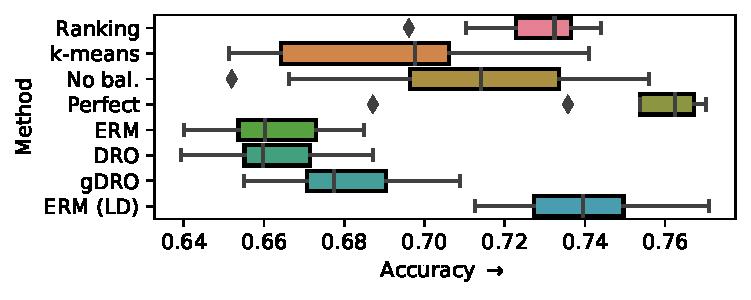
\includegraphics[width=\columnwidth]{figures/adult_partial_acc.pdf}
    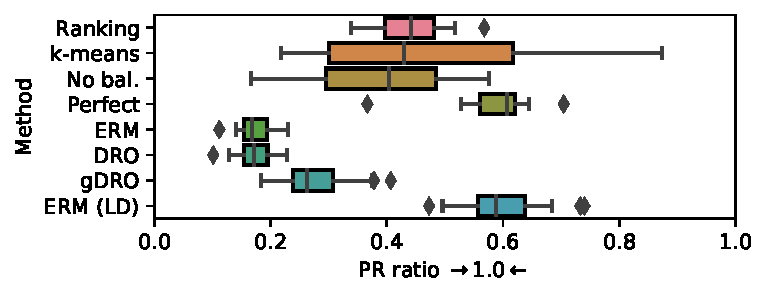
\includegraphics[width=\columnwidth]{figures/adult_partial_prr.pdf}
    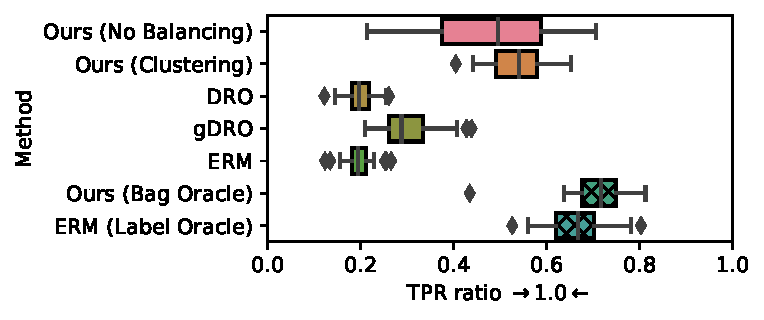
\includegraphics[width=\columnwidth]{figures/adult_partial_tprr.pdf}
    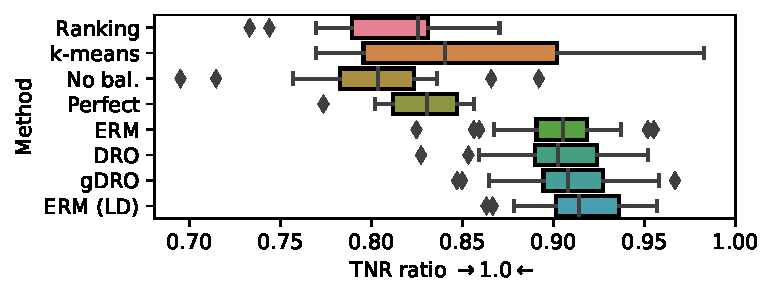
\includegraphics[width=\columnwidth]{figures/adult_partial_tnrr.pdf}
    \caption{%
    Results for the Adult Income dataset with \emph{subgroup bias},
    for the binary classification task of predicting whether an individual earns $>$\$50,000 with a binary subgrouping based on \emph{gender}.
    \texttt{ERM (LD)} refers to a model based on ERM (empirical risk minimization),
    trained on a \emph{l}abelled \emph{d}eployment set; thus not suffering from bias in the training set.
    \textsc{Top left}: Accuracy.
    \textsc{Top right}: Positive rate ratio.
    \textsc{Bottom left}: True positive rate ratio.
    \textsc{Bottom right}: True negative rate ratio.
    For the \texttt{Ranking} clustering, the clustering accuracy was 69.7\% $\pm$ 0.3\%;
    for \texttt{K-means} it was 43\% $\pm$ 3\%.
    }%
    \label{fig:adult-subgroup-bias}
\end{figure*}
\begin{figure*}[p]
    \centering
    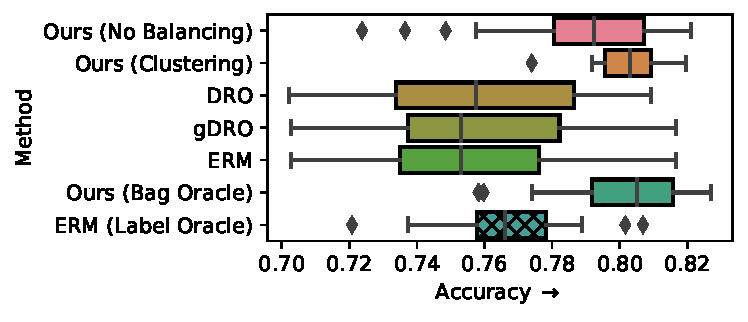
\includegraphics[width=\columnwidth]{figures/adult_miss_s_acc.pdf}
    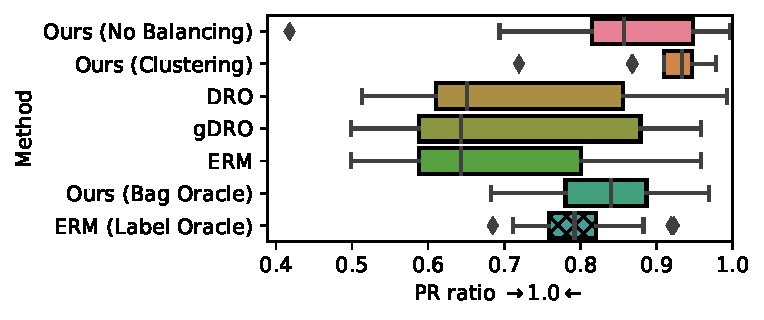
\includegraphics[width=\columnwidth]{figures/adult_miss_s_prr.pdf}
    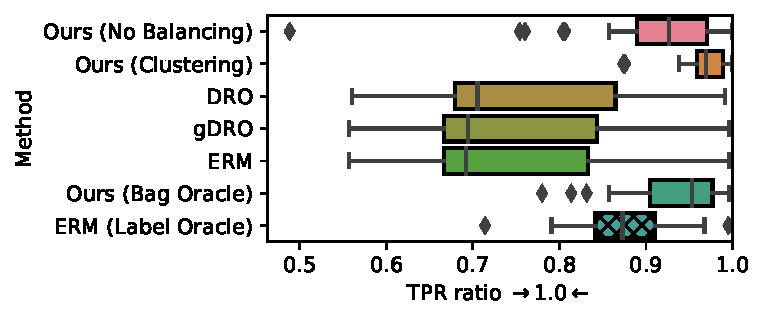
\includegraphics[width=\columnwidth]{figures/adult_miss_s_tprr.pdf}
    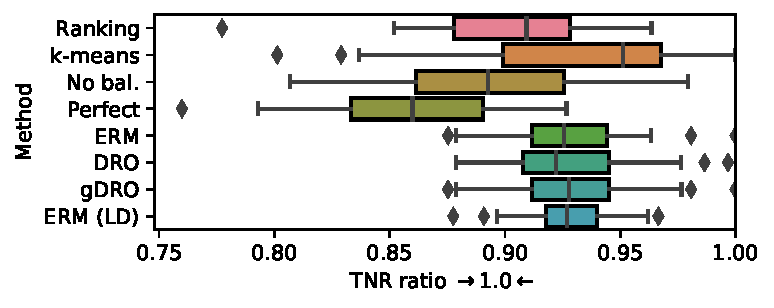
\includegraphics[width=\columnwidth]{figures/adult_miss_s_tnrr.pdf}
    \caption{%
    Results for the Adult Income dataset with a \emph{missing subgroup},
    for the binary classification task of predicting whether an individual earns $>$\$50,000 with a binary subgrouping based on \emph{gender}.
    \texttt{ERM (LD)} refers to a model based on ERM (empirical risk minimization),
    trained on a \emph{l}abelled \emph{d}eployment set; thus not suffering from bias in the training set.
    \textsc{Top left}: Accuracy.
    \textsc{Top right}: Positive rate ratio.
    \textsc{Bottom left}: True positive rate ratio.
    \textsc{Bottom right}: True negative rate ratio.
    For the \texttt{Ranking} clustering, the clustering accuracy was 60.4\% $\pm$ 0.8\%;
    for \texttt{K-means} it was 44\% $\pm$ 3\%.
    }%
    \label{fig:adult-missing-subgroup}
\end{figure*}
Figures~\ref{fig:adult-subgroup-bias} and \ref{fig:adult-missing-subgroup} show results from our method on the Adult Income dataset \cite{Dua:2017}.
This dataset is a common dataset for evaluating fair machine learning models. 
Each instance in the dataset is described by $14$ characteristics including gender, education, marital status, number of work hours per week among others, along with a label denoting income level ($\geq$\$50K or not). 
We transform the representation into $62$ real and binary features along with the subgroup label $s$. %%%%%%%%CHECK THESE VALUES%%%%%%%%%%%% 
The dataset is naturally imbalanced with respect to gender: 30\% of the males are labelled as earning more than \$50K per year (high income), while only 11\% of females are labelled as such.
For further details on the dataset construction, see section~\ref{ssec:dataset-construction-adult}.
%
Following standard practice in algorithmic fairness, e.g. \citet{zemel2013learning}, we consider gender to be the subgroup label $s$.

We study the following two settings.
1) \emph{subgroup bias}: we have labelled training data for males ($s=1$) with both positive and negative outcomes, but for the group of females ($s=0$), we only observe the one-sided negative outcome, so the source $\Omega_{y=1,s=0}$ is missing;
2) \emph{missing subgroup}: we have training data for males with positive and negative outcomes, but do not have labelled data for females, i.e.both \ $\Omega_{y=1,s=0}$ and $\Omega_{y=0,s=0}$ are missing.

As before, \texttt{Ranking}, \texttt{k-means}, \texttt{No bal.}\ and \texttt{Perfect} refer to our method with different procedures for constructing (approximately) perfect bags.
As baseline methods, we have \texttt{ERM} (standard empirical risk minimization with balanced batches), \texttt{DRO} \citep{HasSriNamLia18}, \texttt{gDRO} \citep{sagawa2019distributionally}
and \texttt{ERM (LD)} which is the same model as \texttt{ERM}, but trained on the labelled deployment set, in addition to the training set.

In both settings, we observe the same order as for the other dataset in terms of accuracy: \texttt{Perfect} (with ground truth labels for balancing) achieves the highest performance, followed by \texttt{Ranking}, then \texttt{No bal.}, and finally \texttt{k-means}.
However, for the \emph{missing subgroup} setting, \texttt{Ranking} and \texttt{Perfect} are almost identical and the former performs better in terms of de-biasing metrics.
This decreased reliance on balancing can be explained by the additional supervision that comes with having two sources missing instead of one - in order for the discriminator to distinguish between bags from the deployment set and bags from the training set, the former need only contain \emph{one} of the two missing sources.

Generally, we observe a high variance in the results. This is not attributable to our method, however, with the baselines exhibiting the same behaviour, but rather to the fact that the Adult Income dataset is a very noisy dataset which, at the best of times, allows only about 85\% accuracy to be attained (see also \cite{agrawal2020debiasing}). The problem is that samples vary widely in how informative they are. This, coupled with our artificially biasing the dataset to be even more biased (as \emph{subgroup bias} and \emph{missing subgroup}), makes the achievable performance very dependent on which samples the classifier gets to see, which varies according to the random seed used for the data set split.

\subsection{Dataset Construction}\label{sec:dataset-construction}

\paragraph{Coloured MNIST biasing parameters.}
To simulate a real-word setting where the data, labelled or otherwise, is not naturally balanced, we bias the Coloured MNIST training and deployment sets by downsampling certain colour/digit combinations. The proportions of each such combination \emph{retained} in the \emph{subgroup bias} (in which we have one source missing from the training set) and \emph{missing subgroup} (in which we have two sources missing from the training set) are enumerated in table~\ref{color_mnist_biasing_po} and \ref{color_mnist_biasing_id}, respectively.
For the 3-digit-3-colour variant of the problem, no biasing is applied to either the deployment set or the training set (the missing combinations are specified in the caption accompanying figure~\ref{fig:cmnist-3dig-4miss-add}); this variant was experimented with only under the subgroup-bias setting.

\begin{table}[ht]
\caption{Biasing parameters for the training (left) and deployment (right) sets of Coloured MNIST in the \emph{subgroup bias} setting.}
\label{color_mnist_biasing_po}
\centering
\begin{tabular}{lcc}
\toprule
Combination   & \multicolumn{2}{c}{Proportion retained} \\ \cmidrule(lr){2-3}
  & training set & deployment set \\ \midrule
(y = 2, s = {\color{purple}purple}) & 1.0  & 0.7 \\
(y = 2, s = {\color{green}green})   & 0.3  & 0.4 \\
(y = 4, s = {\color{purple}purple}) & 0.0  & 0.2 \\
(y = 4, s = {\color{green}green})   & 1.0  & 1.0 \\
\bottomrule
\end{tabular}
\end{table}

\begin{table}[ht]
\caption{Biasing parameters for the training (left) and deployment (right) sets of Coloured MNIST in the \emph{missing subgroup} setting.}
\label{color_mnist_biasing_id}
\centering
\begin{tabular}{lcc}
\toprule
Combination   & \multicolumn{2}{c}{Proportion retained} \\ \cmidrule(lr){2-3}
  & training set & deployment set \\ \midrule
(y = 2, s = {\color{purple}purple}) & 0.0  & 0.7 \\
(y = 2, s = {\color{green}green})   & 0.85 & 0.6 \\
(y = 4, s = {\color{purple}purple}) & 0.0  & 0.4 \\
(y = 4, s = {\color{green}green})   & 1.0  & 1.0 \\
\bottomrule
\end{tabular}
\end{table}

\paragraph{Adult Income.}\label{ssec:dataset-construction-adult}
For the Adult Income dataset, we do not need to apply any synthetic biasing as the dataset naturally contains some bias wrt $s$. Thus, we instantiate the deployment set as just a random subset of the original dataset. Explicit balancing of the test set is needed to yield meaningful evaluation, however, namely in the penalizing of biased classifiers, but need be taken in doing so. Balancing the test set such that
\begin{align}
    |\{x \in X |s=0, y=0\}| &= |\{x \in X |s=1, y=0\}|    \nonumber\\
    \text{and}~|\{x \in X |s=0, y=1\}| &= |\{x \in X |s=1, y=1\}|
\end{align}
where for both target classes, $y=0$ and $y=1$, the proportions of the groups $s=0$ and $s=1$ are made to be the same, is intuitive, yet at the same time precludes sensible comparison of the accuracy/fairness trade-off of the different classifiers.
Indeed, with the above conditions, a majority classifier (predicting all 1s or 0s) achieves comparable accuracy to the fairness-unaware baselines, while also yielding perfect fairness, by construction.
This observation motivated us to devise an alternative scheme, where we balance the test set according to the following constraints
\begin{align}
    & |\{x \in X |s=0, y=0\}| 
    = |\{x \in X |s=0, y=1\}|  \nonumber \\
    = &|\{x \in X |s=1, y=1\}|
    = |\{x \in X |s=1, y=0\}|~.
 \end{align}
That is, all subsets of $\gS \times \gY$ are made to be equally sized. Under this new scheme the accuracy of the the majority classifier is 50\% for the binary-classification task.


\subsection{Optimization}
\begin{table*}[p]
 \centering
 \caption{Selected hyperparameters for experiments with Coloured MNIST, Adult and CelebA datasets.}
 \label{tab:hparams}
\scalebox{0.65}{
 \begin{tabular}{llll}
 \toprule
 & \textsc{Coloured MNIST} & \textsc{Adult} & \textsc{CelebA}       
 \\ & 2-dig SB / 2-dig MS / 3-dig SB
 \\ \midrule
 Input size  &   $3 \times 32 \times 32$ & $61$ & $3 \times 64 \times 64$ \\  \midrule
 \multicolumn{4}{c}{Autoencoder}                     \\ \midrule
 Levels                      & $4$         & $1$    & $5$\\
 Level depth                 & $2$         & $1$    & $2$\\
 Hidden units / level        & $[32, 64, 128, 256]$ & $[61]$ & $[32, 64, 128, 256, 512]$\\
 Activation                  & GELU        & GELU   & GELU   \\
 Downsampling op.  & Strided Convs. & -- & Strided Convs.\\
 Reconstruction loss         & MSE         & Mixed$^1$  & MSE \\
 Learning rate               & $1 \times 10^{-3}$   & $1 \times 10^{-3}$  & $1 \times 10^{-3}$ \\ \midrule
 \multicolumn{4}{c}{Clustering}                      \\ \midrule
 Batch size                  & $256$      & $1000$  & --\\
 AE pre-training epochs      & $150$        & $100$ & --   \\
 Clustering epochs           & $100$       & $300$  & -- \\
 Self-supervised loss & Cosine + BCE & Cosine + BCE & --\\
 U (for ranking statistics)             & $5$         & $3$     & --    \\   \midrule
 \multicolumn{4}{c}{Distribution Matching}                   \\ \midrule
 Batch size & $1$/$32$/$14$  & $64$   & $32$ \\
 Bag size   & $256$/$8$/$18$ & $32$ & $8$ \\
 Training iterations    & $8\text{k}/8\text{k}/20\text{k}$ & $5\text{k}$ & $15\text{k}$ \\
 Encoding ($z$) size$^2$  & $128$   & $35$  & $128$ \\
 Binarised $z_s$ & {\boxedsymbols ✗}\, / \cmark\, / \cmark & \xmark & \xmark \\
 $y$-predictor weight ($\lambda_1$) & $1$ & $0$ & $1$  \\ 
 $s$-predictor weight ($\lambda_2$) & $1$ & $0$ & $0$  \\ 
 Adversarial weight ($\lambda_3$)   & $1 \times
 10^{-3}$   & $1$   & $1$\\ 
 Stopgradient $\left(\nabla_\theta h_\psi(f_\theta(X^\mathit{dep}))=0\right)$ & \xmark & \cmark & \xmark \\
 \midrule
 \multicolumn{4}{c}{Predictors}   \\ \midrule
 Learning rate  & $3 \times 10^{-4}$ &   $1 \times 10^{-3}$  $ 1 \times 10^{-3}$\\
 \midrule
 \multicolumn{4}{c}{Discriminator}                   \\ \midrule
 Attention mechanism$^3$    & Gated   & Gated & Gated \\
 Hidden units pre-aggregation  & $[256, 256]$  & $[32]$ & $[256, 256]$\\
 Hidden units post-aggregation & $[256, 256]$ & --  & $[256, 256]$ \\
 Embedding dim (for attention) & $32$ & $128$ & $128$ \\
 Activation & GELU & GELU & GELU \\
 Learning rate  & $3 \times 10^{-4}$    & $1 \times 10^{-3}$ & $1 \times 10^{-3}$\\
 Updates / AE update    & $1$  & $3$    & $1$    \\
 \bottomrule
 \multicolumn{4}{l}{\footnotesize $^1$ Cross-entropy is used for categorical features, MSE for continuous features.} \\
  \multicolumn{4}{p{\textwidth}}{\footnotesize $^2$ $|z|$ denotes the combined size of $z_s$ and $z_y$, with the former occupying $\ceil{\text{log}_2(\mathcal{S})}$ dimensions, the latter the remaining } \\
  \multicolumn{4}{p{\textwidth}}{\footnotesize dimensions.} \\
  \multicolumn{4}{p{\textwidth}}{\footnotesize $^3$ The attention mechanism used for computing the sample-weights within a bag. \emph{Gated} refers to gated attention  proposed by
%   \cite{ilse2018attention}, while \emph{SDP} refers to the scaled dot-product attention proposed by \cite{vaswani2017attention}.
  } \\ 
  \multicolumn{4}{p{\textwidth}}{\footnotesize  \cite{ilse2018attention}.} \\ 
 \end{tabular}
}
\end{table*}

The hyperparameters and architectures for the Autoencoder (\texttt{AE}), Predictor and Discriminator subnetworks used for the experiments with all datasets are detailed in Table \ref{tab:hparams}. All networks are trained using the Adam optimiser \citep{kingma2015adam}.

For the Coloured MNIST and CelebA datasets, the baseline \texttt{CNN}, \texttt{DRO}, and \texttt{LfF} (in the case of the former) models use an architecture identical to that of the encoder with two exceptions: 1) max-pooling being used for spatial downsampling instead of strided convolutions; 2) the final convolutional layer is followed by a global average pooling layer followed by a fully-connected classification layer. For evaluating our method, we simply train a linear classifier on top of $z_y$; this is sufficient due to linear-separability being enforced during training by the $y$-predictor.
For the Adult Income dataset, we use an MLP made up of a single hidden layer 35 units in size, followed by a SELU activation \citep{klambauer2017self}, as both both the downstream classifier for our method, and as the network architecture of the baselines. 
All baselines and downstream classifiers alike were trained for $60$ epochs with a learning rate of $1 \times 10^{-3}$ and a batch size of $256$.

Since, by design, we do not have labels for all subgroups the model will be tested on, and bias against these missing subgroups is what we aim to avoid, properly validating, and thus conducting hyperparameter selection for models generally, is not straightforward.
We can use estimates of the mutual information between the learned-representation and $s$ and $y$ (which we wish to minimise w.r.t.\ to the former, maximise w.r.t.\ the latter) to guide the process, though optimizing the model w.r.t.\ to these metrics obtained from only the training set does not guarantee generalization to the missing subgroups.
We can, however, additionally measure the entropy of the predictions on the encoded test set and seek to maximise it across all samples, or alternatively train a discriminator of the same kind used for distribution matching as a measure the shift in the latent space between datasets.
We use the latter approach (considering, the learned distance between subspace distributions, accuracy, and reconstruction loss) to inform an extensive grid-search over the hyperparameter space of our model.

For the \texttt{DRO} baseline, we allowed access to the labels of the test set for the purpose of hyperparameters selection, performing a grid-search over multiple splits to avoid overfitting to any particular instantiation.
Specifically, the threshold ($\eta$) parameter for \texttt{DRO} was determined by a grid-search over the space $\{0.01, 0.1, 0.3, 1.0\}$. The same procedure was carried out for selecting the model capacity constant ($C$) of the related \texttt{gDRO} baseline.

In addition to the losses stated in the distribution matching objective, $\mathcal{L}$, in the main text, we also regularise the encoder by the $\ell^2$ norm of its embedding, multiplied by a small pre-factor, finding this to work better than more complex regularization methods, such as spectral normalization \citep{miyato2018spectral}, for stabilizing training.

\subsection{Visualizations of results}\label{sec:qual-results}
Figures~\ref{fig:attn_maps} and \ref{fig:cmnist-recon} show some additional visualizations for our results.
For details, see the captions.
\begin{figure*}[tb]
  \centering
    % \begin{subfigure}[b]{0.49\textwidth}
    
\includegraphics[width=0.9\textwidth]{figures/celeba_attn_map.png}
    % \end{subfigure}
    % \hfill
    % \begin{subfigure}[b]{0.49\textwidth}
    
\includegraphics[width=0.9\textwidth]{figures/cmnist_attn_map.png}
    % \end{subfigure}
  \caption{
    Example sample-wise attention maps for bags of CelebA (left) and Coloured MNIST (right) images sampled from a balanced deployment set. The training set is biased according to the SB setting where for CelebA ``smiling females'' constitute the missing source and for Colored MNIST {\color{purple}purple} fours constitute the missing source. The attention weights are used during the discriminator's aggregation step to compute a weighted sum over the bag. The attention-weight assigned to each sample is proportional to the lightness of its frame, with black signifying a weight of 0, white a weight of 1. Those samples belonging to the missing subgroup are assigned the highest weight as they signal from which dataset (training vs. deployment) the bag containing them was drawn from.
  }%
  \label{fig:attn_maps}
\end{figure*}

% \subsection{Qualitative results}\label{sec:qual-results}
\begin{figure*}[tb]
  \centering
  \begin{subfigure}[b]{0.39\textwidth}
    \centering
    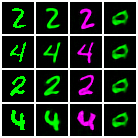
\includegraphics[width=\textwidth]{example_images/fresh-dawn-2179_train_reconstructions_9900.png}
    \caption{
    Different reconstructions on the training set.
    Corresponding to: original, full reconstruction, reconstruction of $z_y$, reconstruction of $z_s$.
    }%
    \label{fig:cmnist-recon-training}
  \end{subfigure}
  % \hfill
  \quad
  \begin{subfigure}[b]{0.39\textwidth}
    \centering
    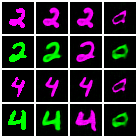
\includegraphics[width=\textwidth]{example_images/fresh-dawn-2179_context_reconstructions_9900.png}
    \caption{
    Different reconstructions on the deployment set.
    Corresponding to: original, full reconstruction, reconstruction of $z_y$, reconstruction of $z_s$.
    }%
    \label{fig:cmnist-recon-deployment}
  \end{subfigure}
  \caption{
   Visualization of our method's solutions for the Coloured MNIST dataset, with {\color{purple}purple} as the missing subgroup.
   In each of the subfigures \ref{fig:cmnist-recon-training} and \ref{fig:cmnist-recon-deployment}:
   Column 1 shows the original images from $x$ from the respective set.
   Column 2 shows plain reconstructions generated from $x_\textit{recon}=g(f_y(x), f_s(x))$.
   Column 3 shows reconstruction with zeroed-out $z_s$: $g(f_y(x), 0)$, which effectively visualises $z_y$.
   Column 4 shows the result of an analogous process where $z_y$ was zeroed out instead.
  }%
  \label{fig:cmnist-recon}
\end{figure*}
% Given a learned invariant representation, we can generate a reconstruction to visualise the information contained in it.
% An example of this can be seen in \figref{fig:3dig-examples}.
% This is from our experiment with 3 digits in Colored MNIST.
% We can clearly see that the reconstructed invariant representation has lost all color information;
% instead all digits are magenta-colored, which was the majority color in the training set.

\subsection{Code}
The code will be published at the following URL: \url{https://github.com/predictive-analytics-lab/fair-dist-matching}.
Instructions on how to run them can be found in the \texttt{README.md}.

\subsection{Additional metrics}
Figures~\ref{fig:cmnist-2v4-partial-add}, \ref{fig:cmnist-2v4-miss-s-add},  and \ref{fig:celeba-gender-smiling-add} show the true positive rate (TPR) ratio and the true negative rate (TNR) ratio as additional metrics for Coloured MNIST (2 digits) and CelebA.
These are computed as the ratio of TPR (or TNR) on subgroup $s=0$ over the TPR (or TNR) on subgroup $s=1$; if this gives a number greater than 1, the inverse is taken.
Similarly to the PR ratio reported in the main paper, these ratios give an indication of how much the prediction of the classifier depends on the subgroup label $s$.

Figure~\ref{fig:cmnist-3dig-4miss-add} shows metrics specific to multi-valued $s$ (\ie, non-binary $s$).
We report the minimum (i.e. farthest away from 1) of the pairwise ratios (PR/TPR/TNR ratio min) as well as the largest difference between the raw values (PR/TPR/TNR diff max) . 
Additionally, we compute the Hirschfeld-Gebelein-R\'enyi (HGR) maximal correlation \citep{renyi1959measures} between $S$ and $Y$, serving as a measure of dependence defined between two variables with arbitrary support.
\begin{figure*}[htp]
  \centering
%   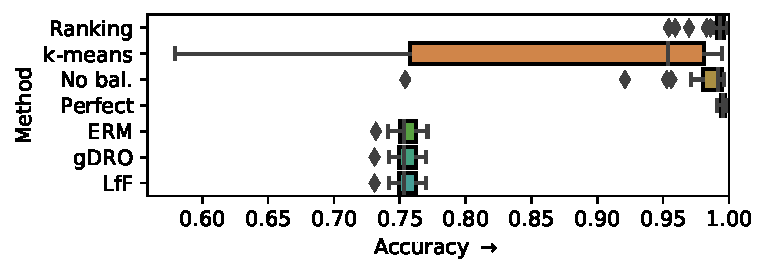
\includegraphics[width=\columnwidth]{figures/cmnist_2v4_partial_acc.pdf}
%   \includegraphics[width=\columnwidth]{figures/cmnist_2v4_partial_pr.pdf}
%   \includegraphics[width=\columnwidth]{figures/cmnist_2v4_partial_tpr.pdf}
%   \includegraphics[width=\columnwidth]{figures/cmnist_2v4_partial_tnr.pdf}
  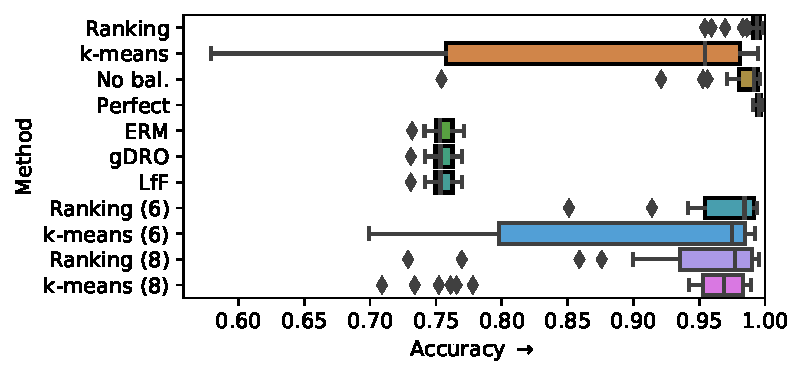
\includegraphics[width=0.8\columnwidth]{figures/cmnist_2v4_partial_overcluster_acc.pdf}
  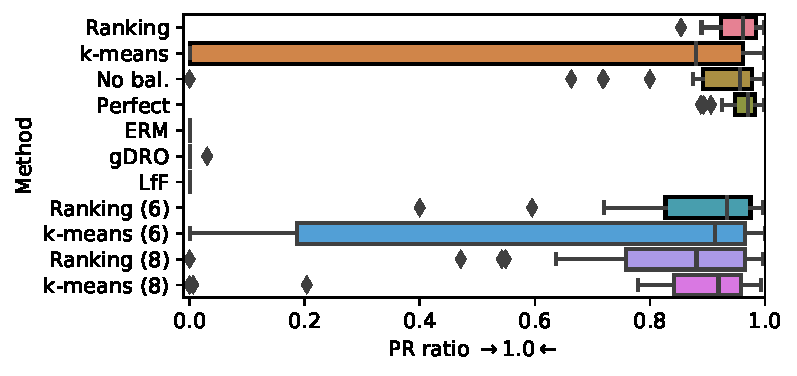
\includegraphics[width=0.8\columnwidth]{figures/cmnist_2v4_partial_overcluster_prr.pdf}
  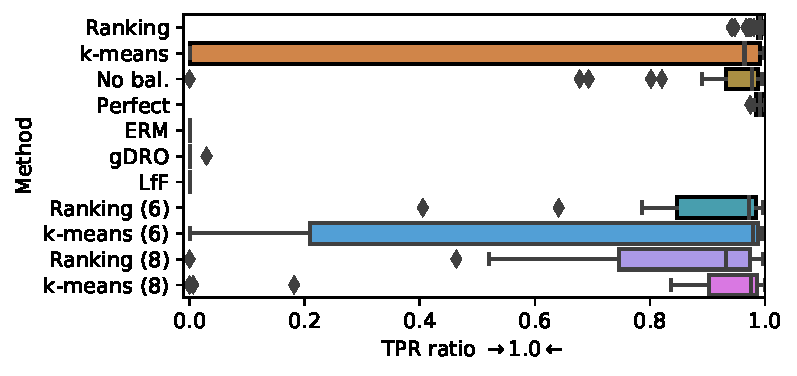
\includegraphics[width=0.8\columnwidth]{figures/cmnist_2v4_partial_overcluster_tprr.pdf}
  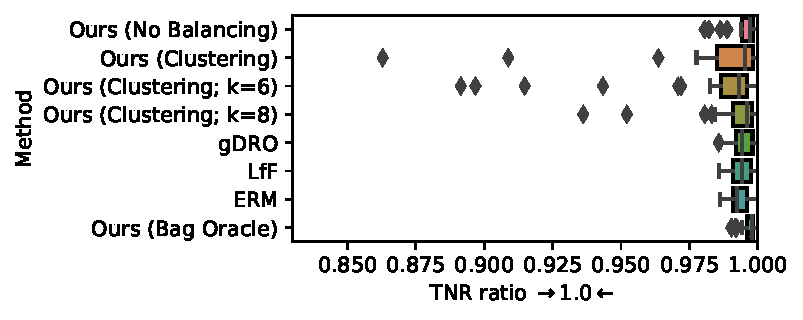
\includegraphics[width=0.8\columnwidth]{figures/cmnist_2v4_partial_overcluster_tnrr.pdf}
  \caption{
    Results from 30 repeats for the Coloured MNIST dataset with two digits, 2 and 4, with \emph{subgroup bias} for the colour `{\color{purple}purple}': for {\color{purple}purple}, only the digit class `2' is present.
    \textsc{Top left}: Accuracy.
    \textsc{Top right}: Positive rate ratio.
    \textsc{Bottom left}: True positive rate ratio.
    \textsc{Bottom right}: True negative rate ratio.
    For the \texttt{Ranking} clustering, the clustering accuracy was 96\% $\pm$ 6\%;
    for \texttt{K-means} it was 64\% $\pm$ 10\%.
    For an explanation of \texttt{Ranking (8)} and \texttt{K-means (8)} see section~\ref{sec:overclustering}.
  }%
  \label{fig:cmnist-2v4-partial-add}
\end{figure*}
\begin{figure*}[htp]
  \centering
%   \includegraphics[width=\columnwidth]{figures/cmnist_2v4_miss_s_alt_acc.pdf}
%   \includegraphics[width=\columnwidth]{figures/cmnist_2v4_miss_s_alt_pr.pdf}
%   \includegraphics[width=\columnwidth]{figures/cmnist_2v4_miss_s_alt_tpr.pdf}
%   \includegraphics[width=\columnwidth]{figures/cmnist_2v4_miss_s_alt_tnr.pdf}
  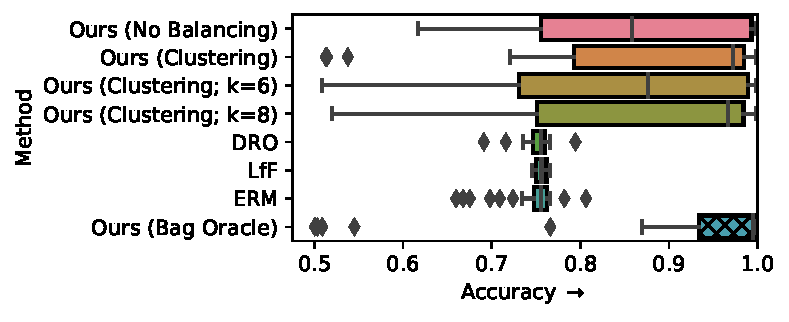
\includegraphics[width=0.8\columnwidth]{figures/cmnist_2v4_miss_s_overcluster_acc.pdf}
  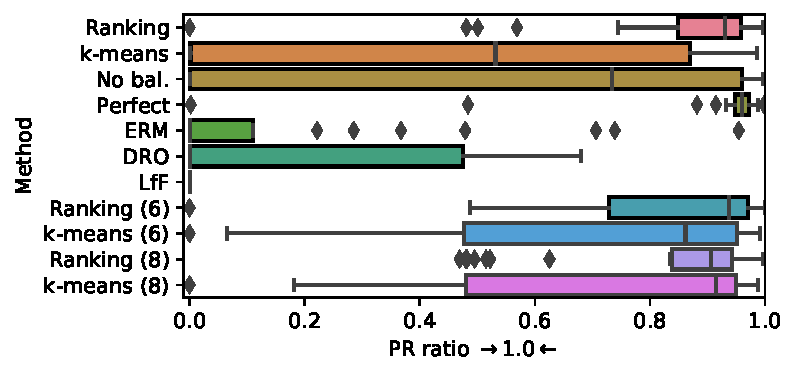
\includegraphics[width=0.8\columnwidth]{figures/cmnist_2v4_miss_s_overcluster_prr.pdf}
  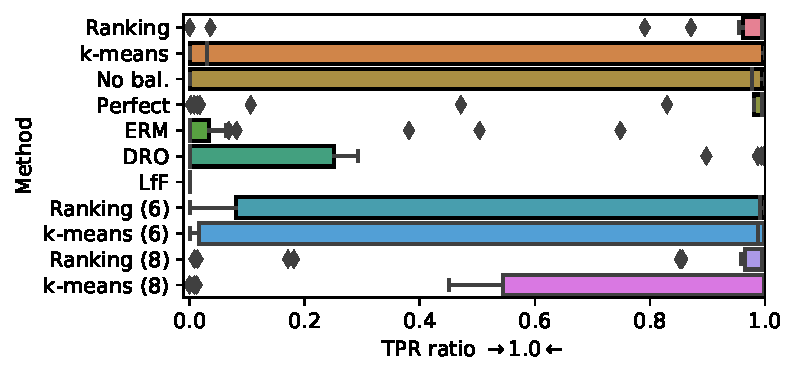
\includegraphics[width=0.8\columnwidth]{figures/cmnist_2v4_miss_s_overcluster_tprr.pdf}
  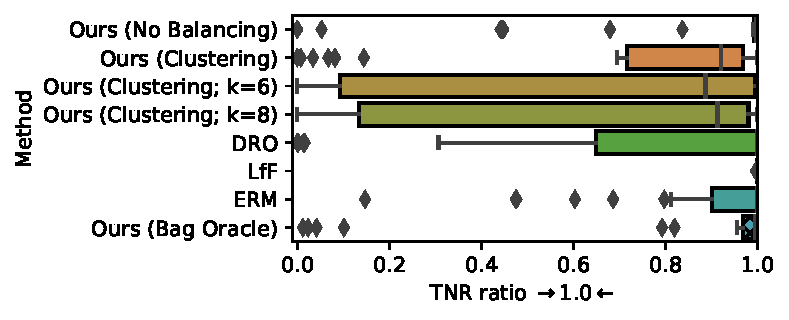
\includegraphics[width=0.8\columnwidth]{figures/cmnist_2v4_miss_s_overcluster_tnrr.pdf}
  \caption{
    Results from 30 repeats for the Coloured MNIST dataset with two digits, 2 and 4, with a \emph{missing subgroup}: the training dataset only has {\color{green}green} digits.
    \textsc{Top left}: Accuracy.
    \textsc{Top right}: Positive rate ratio.
    \textsc{Bottom left}: True positive rate ratio.
    \textsc{Bottom right}: True negative rate ratio.
    For the \texttt{Ranking} clustering, the clustering accuracy was 88\% $\pm$ 5\%;
    for \texttt{K-means} it was 72\% $\pm$ 16\%.
    For an explanation of \texttt{Ranking (8)} and \texttt{K-means (8)} see section~\ref{sec:overclustering}.
  }%
  \label{fig:cmnist-2v4-miss-s-add}
\end{figure*}
\begin{figure*}[htp]
  \centering
%   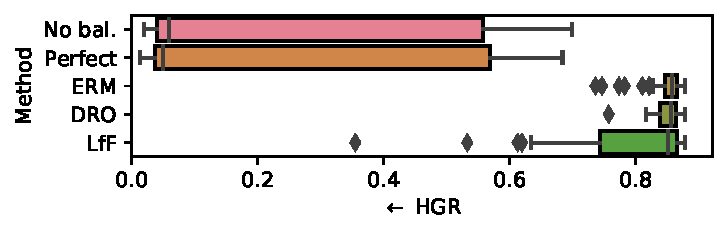
\includegraphics[width=\columnwidth]{figures/cmnist_3dig_4miss_hgr.pdf}\\
  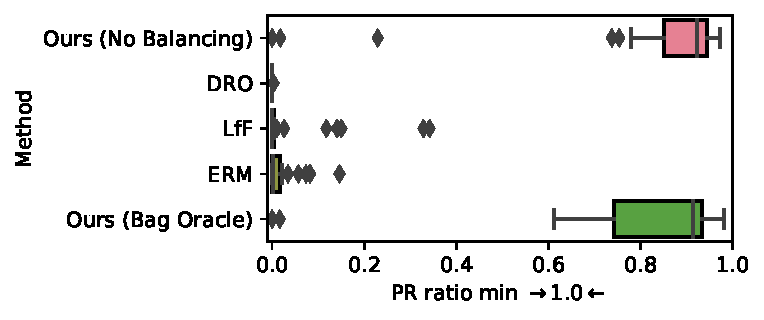
\includegraphics[width=0.8\columnwidth]{figures/cmnist_3dig_4miss_prr-min.pdf}
  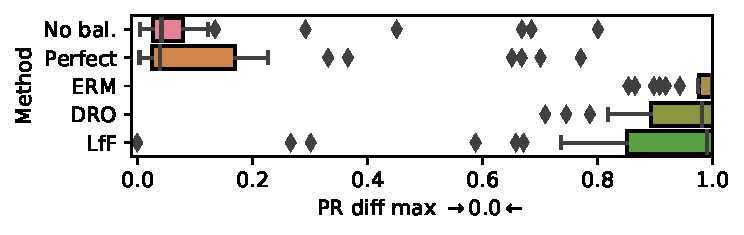
\includegraphics[width=0.8\columnwidth]{figures/cmnist_3dig_4miss_prd-max.pdf}
  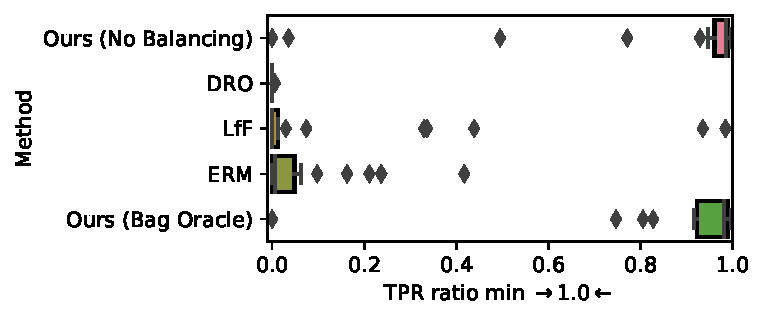
\includegraphics[width=0.8\columnwidth]{figures/cmnist_3dig_4miss_tprr-min.pdf}
  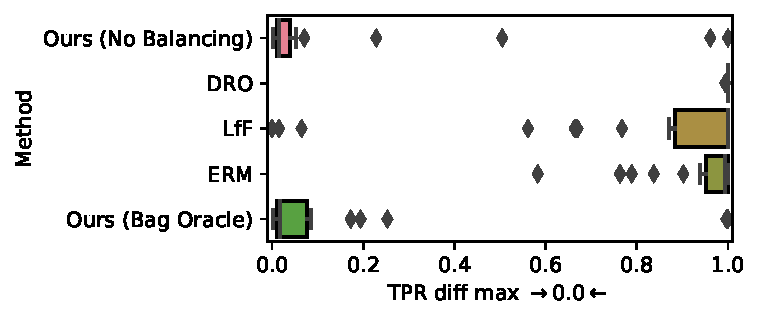
\includegraphics[width=0.8\columnwidth]{figures/cmnist_3dig_4miss_tprd-max.pdf}
  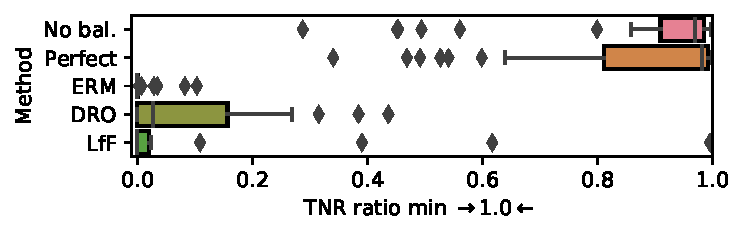
\includegraphics[width=0.8\columnwidth]{figures/cmnist_3dig_4miss_tnrr-min.pdf}
  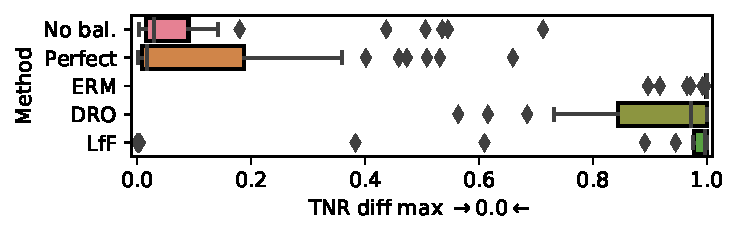
\includegraphics[width=0.8\columnwidth]{figures/cmnist_3dig_4miss_tnrd-max.pdf}
  \caption{
    Results from 30 repeats for the Coloured MNIST dataset with three digits: `2', `4' and `6'.
    Four combinations of digit and colour are missing: {\color{green}green} 2's, {\color{blue}blue} 2's, {\color{blue}blue} 4's and {\color{green}green} 6's.
    % \textsc{First row}: Hirschfeld-Gebelein-R\'enyi maximal correlation between $S$ and $Y$.
    \textsc{First row, left}: minimum of all positive rate ratios.
    \textsc{First row, right}: maximum of all positive rate differences.
    \textsc{Second row, left}: minimum of all true positive rate ratios.
    \textsc{Second row, right}: maximum of all true positive rate differences.
    \textsc{Third row, left}: minimum of all true negative rate ratios.
    \textsc{Third row, right}: maximum of all true negative rate differences.
  }%
  \label{fig:cmnist-3dig-4miss-add}
\end{figure*}
\begin{figure*}[htp]
  \centering
%   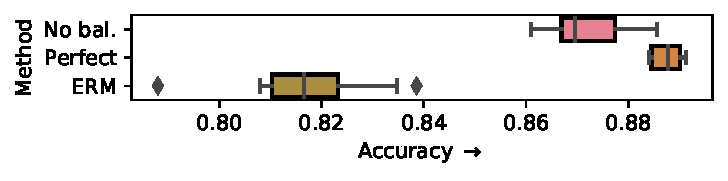
\includegraphics[width=\columnwidth]{figures/celeba_gender_smiling_acc.pdf}
%   \includegraphics[width=\columnwidth]{figures/celeba_gender_smiling_pr.pdf}
  \includegraphics[width=\columnwidth]{figures/celeba_gender_smiling_tprr.pdf}
  \includegraphics[width=\columnwidth]{figures/celeba_gender_smiling_tnrr.pdf}
  \caption{
    Results from 10 repeats for the CelebA dataset with the \emph{subgroup bias} setting.
    The task is to predict ``smiling'' vs ``non-smiling'' and the subgroups are based on gender.
    The subgroup ``female'' is missing samples for the ``smiling'' class.
    % \textsc{Top left}: Accuracy.
    % \textsc{Top right}: Positive rate ratio.
    \textsc{Left}: True positive rate ratio.
    \textsc{Right}: True negative rate ratio.
  }%
  \label{fig:celeba-gender-smiling-add}
\end{figure*}

\subsection{Clustering with an incorrect number of clusters}\label{sec:overclustering}
We also investigate what happens when the number of clusters is set incorrectly.
For 2-digit Coloured MNIST, we expect 4 clusters, corresponding to the 4 possible combinations of the binary class label $y$ and the binary subgroup label $s$.
However, there might be circumstances where the correct number of clusters is not known; how does the batch balancing work in this case?
We run experiments with the number of clusters set to 6 and to 8, while otherwise not changing any part of the method.
It should be noted that this is a very na\"ive way of dealing with an unknown number of clusters.
There are methods specifically designed for identifying the right number of clusters \citep{hamerly2004learning,chazal2013persistence},
and that is what would be used if this situation came up in practice.

The results can be found in figures~\ref{fig:cmnist-2v4-partial-add} and \ref{fig:cmnist-2v4-miss-s-add}.
Bags and batches are constructed by drawing an equal number of samples from each cluster.
Unsurprisingly, the method performs worse than with the correct number of clusters.
When investigating how the clustering methods deal with the larger number of clusters,
we found that it is predominantly those samples that do not appear in the training set
which get spread out among the additional clusters.
This is most likely due to the fact that the clustering is semi-supervised,
with those clusters that occur in the training set having supervision.
The overall effect is that the samples which are not appearing in the training set are overrepresented in the drawn bags,
which means it is easier for the adversary to identify where the bags came from,
and the encoder cannot properly learn to produce an invariant encoding.

% \begin{table*}[tp]
%   \centering
%   \caption{
%     Results on Colored MNIST dataset for a 3-digits-3-colors task, i.e. classification of the digits \emph{two} versus \emph{four} vs \emph{six} with a protected attribute that can take three values ({\color{purple}purple}, {\color{green}green}, {\color{blue}blue}).
%     We consider the scenarios of learning with subgroup bias with four sources missing (30 repeats). 
%   }
%   \label{tab:colormnist3_sup}
%   \scalebox{0.79}{
%   \begin{tabular}{lccccccc}
%     \hline
%     \multicolumn{6}{c}{}\\
%     \multicolumn{6}{c}{Learning with subgroup bias, the sources
%     $\mathcal{M}_{y=\text{'two'},s=\color{green}green}$,
%     $\mathcal{M}_{y=\text{'two'},s=\color{blue}blue}$,
%     $\mathcal{M}_{y=\text{'four'},s=\color{blue}blue}$ and
%     $\mathcal{M}_{y=\text{'six'},s=\color{green}green}$
%     are invisible.}\\
%     \multicolumn{6}{c}{}\\
%     \hline
%     %
%                                          &         AR min. ratio& TPR min. ratio & TNR min. ratio &   AR max. diff &  TPR max. diff &   TNR max. diff \\
%                              \texttt{ZSF} &    0.604 $\pm$ 0.213 &  0.866 $\pm$ 0.176 &  0.702 $\pm$ 0.292 &  0.236 $\pm$ 0.189 &  0.133 $\pm$ 0.175 &  0.297 $\pm$ 0.291 \\
%  \texttt{DRO \cite{HasSriNamLia18}} &     0.027 $\pm$ 0.05 &  0.077 $\pm$ 0.145 &  0.128 $\pm$ 0.147 &  0.887 $\pm$ 0.101 &  0.923 $\pm$ 0.145 &  0.871 $\pm$ 0.147 \\
%   \texttt{Kamiran \& Calders (2012) CNN} &    0.072 $\pm$ 0.077 &  0.208 $\pm$ 0.217 &  0.039 $\pm$ 0.054 &  0.904 $\pm$ 0.087 &  0.792 $\pm$ 0.217 &  0.961 $\pm$ 0.054 \\
%     \hline
%     \hline
%   \end{tabular}}
% \vspace{-0.5cm}
% \end{table*}
% \bibliography{bibfile}
% \bibliographystyle{icml2021}
% \end{document}

% \FloatBarrier%
% \clearpage

% \printbibliography%
% \end{refsection}

% \end{document}
